\documentclass{report}

%%%%%%%%%%%%%%%%%%%%%%%%%%%%%%%%%
% PACKAGE IMPORTS
%%%%%%%%%%%%%%%%%%%%%%%%%%%%%%%%%


\usepackage[tmargin=2cm,rmargin=1in,lmargin=1in,margin=0.85in,bmargin=2cm,footskip=.2in]{geometry}
\usepackage{amsmath,amsfonts,amsthm,amssymb,mathtools}
\usepackage[varbb]{newpxmath}
\usepackage{xfrac}
\usepackage[makeroom]{cancel}
\usepackage{mathtools}
\usepackage{bookmark}
\usepackage{enumitem}
\usepackage{hyperref,theoremref}
\hypersetup{
	pdftitle={Assignment},
	colorlinks=true, linkcolor=doc!90,
	bookmarksnumbered=true,
	bookmarksopen=true
}
\usepackage[most,many,breakable]{tcolorbox}
\usepackage{xcolor}
\usepackage{varwidth}
\usepackage{varwidth}
\usepackage{etoolbox}
%\usepackage{authblk}
\usepackage{nameref}
\usepackage{multicol,array}
\usepackage{tikz-cd}
\usepackage[ruled,vlined,linesnumbered]{algorithm2e}
\usepackage{comment} % enables the use of multi-line comments (\ifx \fi) 
\usepackage{import}
\usepackage{xifthen}
\usepackage{pdfpages}
\usepackage{transparent}

\newcommand\mycommfont[1]{\footnotesize\ttfamily\textcolor{blue}{#1}}
\SetCommentSty{mycommfont}
\newcommand{\incfig}[1]{%
    \def\svgwidth{\columnwidth}
    \import{./figures/}{#1.pdf_tex}
}

\usepackage{tikzsymbols}
\renewcommand\qedsymbol{$\Laughey$}


%\usepackage{import}
%\usepackage{xifthen}
%\usepackage{pdfpages}
%\usepackage{transparent}


%%%%%%%%%%%%%%%%%%%%%%%%%%%%%%
% SELF MADE COLORS
%%%%%%%%%%%%%%%%%%%%%%%%%%%%%%



\definecolor{myg}{RGB}{56, 140, 70}
\definecolor{myb}{RGB}{45, 111, 177}
\definecolor{myr}{RGB}{199, 68, 64}
\definecolor{mytheorembg}{HTML}{F2F2F9}
\definecolor{mytheoremfr}{HTML}{00007B}
\definecolor{mylenmabg}{HTML}{FFFAF8}
\definecolor{mylenmafr}{HTML}{983b0f}
\definecolor{mypropbg}{HTML}{f2fbfc}
\definecolor{mypropfr}{HTML}{191971}
\definecolor{myexamplebg}{HTML}{F2FBF8}
\definecolor{myexamplefr}{HTML}{88D6D1}
\definecolor{myexampleti}{HTML}{2A7F7F}
\definecolor{mydefinitbg}{HTML}{E5E5FF}
\definecolor{mydefinitfr}{HTML}{3F3FA3}
\definecolor{notesgreen}{RGB}{0,162,0}
\definecolor{myp}{RGB}{197, 92, 212}
\definecolor{mygr}{HTML}{2C3338}
\definecolor{myred}{RGB}{127,0,0}
\definecolor{myyellow}{RGB}{169,121,69}
\definecolor{myexercisebg}{HTML}{F2FBF8}
\definecolor{myexercisefg}{HTML}{88D6D1}


%%%%%%%%%%%%%%%%%%%%%%%%%%%%
% TCOLORBOX SETUPS
%%%%%%%%%%%%%%%%%%%%%%%%%%%%

\setlength{\parindent}{1cm}
%================================
% THEOREM BOX
%================================

\tcbuselibrary{theorems,skins,hooks}
\newtcbtheorem[number within=section]{Theorem}{Theorem}
{%
	enhanced,
	breakable,
	colback = mytheorembg,
	frame hidden,
	boxrule = 0sp,
	borderline west = {2pt}{0pt}{mytheoremfr},
	sharp corners,
	detach title,
	before upper = \tcbtitle\par\smallskip,
	coltitle = mytheoremfr,
	fonttitle = \bfseries\sffamily,
	description font = \mdseries,
	separator sign none,
	segmentation style={solid, mytheoremfr},
}
{th}

\tcbuselibrary{theorems,skins,hooks}
\newtcbtheorem[number within=chapter]{theorem}{Theorem}
{%
	enhanced,
	breakable,
	colback = mytheorembg,
	frame hidden,
	boxrule = 0sp,
	borderline west = {2pt}{0pt}{mytheoremfr},
	sharp corners,
	detach title,
	before upper = \tcbtitle\par\smallskip,
	coltitle = mytheoremfr,
	fonttitle = \bfseries\sffamily,
	description font = \mdseries,
	separator sign none,
	segmentation style={solid, mytheoremfr},
}
{th}


\tcbuselibrary{theorems,skins,hooks}
\newtcolorbox{Theoremcon}
{%
	enhanced
	,breakable
	,colback = mytheorembg
	,frame hidden
	,boxrule = 0sp
	,borderline west = {2pt}{0pt}{mytheoremfr}
	,sharp corners
	,description font = \mdseries
	,separator sign none
}

%================================
% Corollery
%================================
\tcbuselibrary{theorems,skins,hooks}
\newtcbtheorem[number within=section]{Corollary}{Corollary}
{%
	enhanced
	,breakable
	,colback = myp!10
	,frame hidden
	,boxrule = 0sp
	,borderline west = {2pt}{0pt}{myp!85!black}
	,sharp corners
	,detach title
	,before upper = \tcbtitle\par\smallskip
	,coltitle = myp!85!black
	,fonttitle = \bfseries\sffamily
	,description font = \mdseries
	,separator sign none
	,segmentation style={solid, myp!85!black}
}
{th}
\tcbuselibrary{theorems,skins,hooks}
\newtcbtheorem[number within=chapter]{corollary}{Corollary}
{%
	enhanced
	,breakable
	,colback = myp!10
	,frame hidden
	,boxrule = 0sp
	,borderline west = {2pt}{0pt}{myp!85!black}
	,sharp corners
	,detach title
	,before upper = \tcbtitle\par\smallskip
	,coltitle = myp!85!black
	,fonttitle = \bfseries\sffamily
	,description font = \mdseries
	,separator sign none
	,segmentation style={solid, myp!85!black}
}
{th}


%================================
% LENMA
%================================

\tcbuselibrary{theorems,skins,hooks}
\newtcbtheorem[number within=section]{Lenma}{Lenma}
{%
	enhanced,
	breakable,
	colback = mylenmabg,
	frame hidden,
	boxrule = 0sp,
	borderline west = {2pt}{0pt}{mylenmafr},
	sharp corners,
	detach title,
	before upper = \tcbtitle\par\smallskip,
	coltitle = mylenmafr,
	fonttitle = \bfseries\sffamily,
	description font = \mdseries,
	separator sign none,
	segmentation style={solid, mylenmafr},
}
{th}

\tcbuselibrary{theorems,skins,hooks}
\newtcbtheorem[number within=chapter]{lenma}{Lenma}
{%
	enhanced,
	breakable,
	colback = mylenmabg,
	frame hidden,
	boxrule = 0sp,
	borderline west = {2pt}{0pt}{mylenmafr},
	sharp corners,
	detach title,
	before upper = \tcbtitle\par\smallskip,
	coltitle = mylenmafr,
	fonttitle = \bfseries\sffamily,
	description font = \mdseries,
	separator sign none,
	segmentation style={solid, mylenmafr},
}
{th}


%================================
% PROPOSITION
%================================

\tcbuselibrary{theorems,skins,hooks}
\newtcbtheorem[number within=section]{Prop}{Proposition}
{%
	enhanced,
	breakable,
	colback = mypropbg,
	frame hidden,
	boxrule = 0sp,
	borderline west = {2pt}{0pt}{mypropfr},
	sharp corners,
	detach title,
	before upper = \tcbtitle\par\smallskip,
	coltitle = mypropfr,
	fonttitle = \bfseries\sffamily,
	description font = \mdseries,
	separator sign none,
	segmentation style={solid, mypropfr},
}
{th}

\tcbuselibrary{theorems,skins,hooks}
\newtcbtheorem[number within=chapter]{prop}{Proposition}
{%
	enhanced,
	breakable,
	colback = mypropbg,
	frame hidden,
	boxrule = 0sp,
	borderline west = {2pt}{0pt}{mypropfr},
	sharp corners,
	detach title,
	before upper = \tcbtitle\par\smallskip,
	coltitle = mypropfr,
	fonttitle = \bfseries\sffamily,
	description font = \mdseries,
	separator sign none,
	segmentation style={solid, mypropfr},
}
{th}


%================================
% CLAIM
%================================

\tcbuselibrary{theorems,skins,hooks}
\newtcbtheorem[number within=section]{claim}{Claim}
{%
	enhanced
	,breakable
	,colback = myg!10
	,frame hidden
	,boxrule = 0sp
	,borderline west = {2pt}{0pt}{myg}
	,sharp corners
	,detach title
	,before upper = \tcbtitle\par\smallskip
	,coltitle = myg!85!black
	,fonttitle = \bfseries\sffamily
	,description font = \mdseries
	,separator sign none
	,segmentation style={solid, myg!85!black}
}
{th}



%================================
% Exercise
%================================

\tcbuselibrary{theorems,skins,hooks}
\newtcbtheorem[number within=section]{Exercise}{Exercise}
{%
	enhanced,
	breakable,
	colback = myexercisebg,
	frame hidden,
	boxrule = 0sp,
	borderline west = {2pt}{0pt}{myexercisefg},
	sharp corners,
	detach title,
	before upper = \tcbtitle\par\smallskip,
	coltitle = myexercisefg,
	fonttitle = \bfseries\sffamily,
	description font = \mdseries,
	separator sign none,
	segmentation style={solid, myexercisefg},
}
{th}

\tcbuselibrary{theorems,skins,hooks}
\newtcbtheorem[number within=chapter]{exercise}{Exercise}
{%
	enhanced,
	breakable,
	colback = myexercisebg,
	frame hidden,
	boxrule = 0sp,
	borderline west = {2pt}{0pt}{myexercisefg},
	sharp corners,
	detach title,
	before upper = \tcbtitle\par\smallskip,
	coltitle = myexercisefg,
	fonttitle = \bfseries\sffamily,
	description font = \mdseries,
	separator sign none,
	segmentation style={solid, myexercisefg},
}
{th}

%================================
% EXAMPLE BOX
%================================

\newtcbtheorem[number within=section]{Example}{Example}
{%
	colback = myexamplebg
	,breakable
	,colframe = myexamplefr
	,coltitle = myexampleti
	,boxrule = 1pt
	,sharp corners
	,detach title
	,before upper=\tcbtitle\par\smallskip
	,fonttitle = \bfseries
	,description font = \mdseries
	,separator sign none
	,description delimiters parenthesis
}
{ex}

\newtcbtheorem[number within=chapter]{example}{Example}
{%
	colback = myexamplebg
	,breakable
	,colframe = myexamplefr
	,coltitle = myexampleti
	,boxrule = 1pt
	,sharp corners
	,detach title
	,before upper=\tcbtitle\par\smallskip
	,fonttitle = \bfseries
	,description font = \mdseries
	,separator sign none
	,description delimiters parenthesis
}
{ex}

%================================
% DEFINITION BOX
%================================

\newtcbtheorem[number within=section]{Definition}{Definition}{enhanced,
	before skip=2mm,after skip=2mm, colback=red!5,colframe=red!80!black,boxrule=0.5mm,
	attach boxed title to top left={xshift=1cm,yshift*=1mm-\tcboxedtitleheight}, varwidth boxed title*=-3cm,
	boxed title style={frame code={
					\path[fill=tcbcolback]
					([yshift=-1mm,xshift=-1mm]frame.north west)
					arc[start angle=0,end angle=180,radius=1mm]
					([yshift=-1mm,xshift=1mm]frame.north east)
					arc[start angle=180,end angle=0,radius=1mm];
					\path[left color=tcbcolback!60!black,right color=tcbcolback!60!black,
						middle color=tcbcolback!80!black]
					([xshift=-2mm]frame.north west) -- ([xshift=2mm]frame.north east)
					[rounded corners=1mm]-- ([xshift=1mm,yshift=-1mm]frame.north east)
					-- (frame.south east) -- (frame.south west)
					-- ([xshift=-1mm,yshift=-1mm]frame.north west)
					[sharp corners]-- cycle;
				},interior engine=empty,
		},
	fonttitle=\bfseries,
	title={#2},#1}{def}
\newtcbtheorem[number within=chapter]{definition}{Definition}{enhanced,
	before skip=2mm,after skip=2mm, colback=red!5,colframe=red!80!black,boxrule=0.5mm,
	attach boxed title to top left={xshift=1cm,yshift*=1mm-\tcboxedtitleheight}, varwidth boxed title*=-3cm,
	boxed title style={frame code={
					\path[fill=tcbcolback]
					([yshift=-1mm,xshift=-1mm]frame.north west)
					arc[start angle=0,end angle=180,radius=1mm]
					([yshift=-1mm,xshift=1mm]frame.north east)
					arc[start angle=180,end angle=0,radius=1mm];
					\path[left color=tcbcolback!60!black,right color=tcbcolback!60!black,
						middle color=tcbcolback!80!black]
					([xshift=-2mm]frame.north west) -- ([xshift=2mm]frame.north east)
					[rounded corners=1mm]-- ([xshift=1mm,yshift=-1mm]frame.north east)
					-- (frame.south east) -- (frame.south west)
					-- ([xshift=-1mm,yshift=-1mm]frame.north west)
					[sharp corners]-- cycle;
				},interior engine=empty,
		},
	fonttitle=\bfseries,
	title={#2},#1}{def}



%================================
% Solution BOX
%================================

\makeatletter
\newtcbtheorem{question}{Question}{enhanced,
	breakable,
	colback=white,
	colframe=myb!80!black,
	attach boxed title to top left={yshift*=-\tcboxedtitleheight},
	fonttitle=\bfseries,
	title={#2},
	boxed title size=title,
	boxed title style={%
			sharp corners,
			rounded corners=northwest,
			colback=tcbcolframe,
			boxrule=0pt,
		},
	underlay boxed title={%
			\path[fill=tcbcolframe] (title.south west)--(title.south east)
			to[out=0, in=180] ([xshift=5mm]title.east)--
			(title.center-|frame.east)
			[rounded corners=\kvtcb@arc] |-
			(frame.north) -| cycle;
		},
	#1
}{def}
\makeatother

%================================
% SOLUTION BOX
%================================

\makeatletter
\newtcolorbox{solution}{enhanced,
	breakable,
	colback=white,
	colframe=myg!80!black,
	attach boxed title to top left={yshift*=-\tcboxedtitleheight},
	title=Solution,
	boxed title size=title,
	boxed title style={%
			sharp corners,
			rounded corners=northwest,
			colback=tcbcolframe,
			boxrule=0pt,
		},
	underlay boxed title={%
			\path[fill=tcbcolframe] (title.south west)--(title.south east)
			to[out=0, in=180] ([xshift=5mm]title.east)--
			(title.center-|frame.east)
			[rounded corners=\kvtcb@arc] |-
			(frame.north) -| cycle;
		},
}
\makeatother

%================================
% Question BOX
%================================

\makeatletter
\newtcbtheorem{qstion}{Question}{enhanced,
	breakable,
	colback=white,
	colframe=mygr,
	attach boxed title to top left={yshift*=-\tcboxedtitleheight},
	fonttitle=\bfseries,
	title={#2},
	boxed title size=title,
	boxed title style={%
			sharp corners,
			rounded corners=northwest,
			colback=tcbcolframe,
			boxrule=0pt,
		},
	underlay boxed title={%
			\path[fill=tcbcolframe] (title.south west)--(title.south east)
			to[out=0, in=180] ([xshift=5mm]title.east)--
			(title.center-|frame.east)
			[rounded corners=\kvtcb@arc] |-
			(frame.north) -| cycle;
		},
	#1
}{def}
\makeatother

\newtcbtheorem[number within=chapter]{wconc}{Wrong Concept}{
	breakable,
	enhanced,
	colback=white,
	colframe=myr,
	arc=0pt,
	outer arc=0pt,
	fonttitle=\bfseries\sffamily\large,
	colbacktitle=myr,
	attach boxed title to top left={},
	boxed title style={
			enhanced,
			skin=enhancedfirst jigsaw,
			arc=3pt,
			bottom=0pt,
			interior style={fill=myr}
		},
	#1
}{def}



%================================
% NOTE BOX
%================================

\usetikzlibrary{arrows,calc,shadows.blur}
\tcbuselibrary{skins}
\newtcolorbox{note}[1][]{%
	enhanced jigsaw,
	colback=gray!20!white,%
	colframe=gray!80!black,
	size=small,
	boxrule=1pt,
	title=\textbf{Note:-},
	halign title=flush center,
	coltitle=black,
	breakable,
	drop shadow=black!50!white,
	attach boxed title to top left={xshift=1cm,yshift=-\tcboxedtitleheight/2,yshifttext=-\tcboxedtitleheight/2},
	minipage boxed title=1.5cm,
	boxed title style={%
			colback=white,
			size=fbox,
			boxrule=1pt,
			boxsep=2pt,
			underlay={%
					\coordinate (dotA) at ($(interior.west) + (-0.5pt,0)$);
					\coordinate (dotB) at ($(interior.east) + (0.5pt,0)$);
					\begin{scope}
						\clip (interior.north west) rectangle ([xshift=3ex]interior.east);
						\filldraw [white, blur shadow={shadow opacity=60, shadow yshift=-.75ex}, rounded corners=2pt] (interior.north west) rectangle (interior.south east);
					\end{scope}
					\begin{scope}[gray!80!black]
						\fill (dotA) circle (2pt);
						\fill (dotB) circle (2pt);
					\end{scope}
				},
		},
	#1,
}

%%%%%%%%%%%%%%%%%%%%%%%%%%%%%%
% SELF MADE COMMANDS
%%%%%%%%%%%%%%%%%%%%%%%%%%%%%%


\newcommand{\thm}[2]{\begin{Theorem}{#1}{}#2\end{Theorem}}
\newcommand{\cor}[2]{\begin{Corollary}{#1}{}#2\end{Corollary}}
\newcommand{\mlenma}[2]{\begin{Lenma}{#1}{}#2\end{Lenma}}
\newcommand{\mprop}[2]{\begin{Prop}{#1}{}#2\end{Prop}}
\newcommand{\clm}[3]{\begin{claim}{#1}{#2}#3\end{claim}}
\newcommand{\wc}[2]{\begin{wconc}{#1}{}\setlength{\parindent}{1cm}#2\end{wconc}}
\newcommand{\thmcon}[1]{\begin{Theoremcon}{#1}\end{Theoremcon}}
\newcommand{\ex}[2]{\begin{Example}{#1}{}#2\end{Example}}
\newcommand{\dfn}[2]{\begin{Definition}[colbacktitle=red!75!black]{#1}{}#2\end{Definition}}
\newcommand{\dfnc}[2]{\begin{definition}[colbacktitle=red!75!black]{#1}{}#2\end{definition}}
\newcommand{\qs}[2]{\begin{question}{#1}{}#2\end{question}}
\newcommand{\pf}[2]{\begin{myproof}[#1]#2\end{myproof}}
\newcommand{\nt}[1]{\begin{note}#1\end{note}}
\newcommand{\mat}[1]{\begin{bmatrix} #1 \end{bmatrix}}
\newcommand{\vect}[1]{\begin{bmatrix} #1 \end{bmatrix}}

\newcommand*\circled[1]{\tikz[baseline=(char.base)]{
		\node[shape=circle,draw,inner sep=1pt] (char) {#1};}}
\newcommand\getcurrentref[1]{%
	\ifnumequal{\value{#1}}{0}
	{??}
	{\the\value{#1}}%
}
\newcommand{\getCurrentSectionNumber}{\getcurrentref{section}}
\newenvironment{myproof}[1][\proofname]{%
	\proof[\bfseries #1: ]%
}{\endproof}

\newcommand{\mclm}[2]{\begin{myclaim}[#1]#2\end{myclaim}}
\newenvironment{myclaim}[1][\claimname]{\proof[\bfseries #1: ]}{}

\newcounter{mylabelcounter}

\makeatletter
\newcommand{\setword}[2]{%
	\phantomsection
	#1\def\@currentlabel{\unexpanded{#1}}\label{#2}%
}
\makeatother




\tikzset{
	symbol/.style={
			draw=none,
			every to/.append style={
					edge node={node [sloped, allow upside down, auto=false]{$#1$}}}
		}
}


% deliminators
\DeclarePairedDelimiter{\abs}{\lvert}{\rvert}
\DeclarePairedDelimiter{\norm}{\lVert}{\rVert}

\DeclarePairedDelimiter{\ceil}{\lceil}{\rceil}
\DeclarePairedDelimiter{\floor}{\lfloor}{\rfloor}
\DeclarePairedDelimiter{\round}{\lfloor}{\rceil}

\newsavebox\diffdbox
\newcommand{\slantedromand}{{\mathpalette\makesl{d}}}
\newcommand{\makesl}[2]{%
\begingroup
\sbox{\diffdbox}{$\mathsurround=0pt#1\mathrm{#2}$}%
\pdfsave
\pdfsetmatrix{1 0 0.2 1}%
\rlap{\usebox{\diffdbox}}%
\pdfrestore
\hskip\wd\diffdbox
\endgroup
}
\newcommand{\dd}[1][]{\ensuremath{\mathop{}\!\ifstrempty{#1}{%
\slantedromand\@ifnextchar^{\hspace{0.2ex}}{\hspace{0.1ex}}}%
{\slantedromand\hspace{0.2ex}^{#1}}}}
\ProvideDocumentCommand\dv{o m g}{%
  \ensuremath{%
    \IfValueTF{#3}{%
      \IfNoValueTF{#1}{%
        \frac{\dd #2}{\dd #3}%
      }{%
        \frac{\dd^{#1} #2}{\dd #3^{#1}}%
      }%
    }{%
      \IfNoValueTF{#1}{%
        \frac{\dd}{\dd #2}%
      }{%
        \frac{\dd^{#1}}{\dd #2^{#1}}%
      }%
    }%
  }%
}
\providecommand*{\pdv}[3][]{\frac{\partial^{#1}#2}{\partial#3^{#1}}}
%  - others
\DeclareMathOperator{\Lap}{\mathcal{L}}
\DeclareMathOperator{\Var}{Var} % varience
\DeclareMathOperator{\Cov}{Cov} % covarience
\DeclareMathOperator{\E}{E} % expected

% Since the amsthm package isn't loaded

% I prefer the slanted \leq
\let\oldleq\leq % save them in case they're every wanted
\let\oldgeq\geq
\renewcommand{\leq}{\leqslant}
\renewcommand{\geq}{\geqslant}

% % redefine matrix env to allow for alignment, use r as default
% \renewcommand*\env@matrix[1][r]{\hskip -\arraycolsep
%     \let\@ifnextchar\new@ifnextchar
%     \array{*\c@MaxMatrixCols #1}}


%\usepackage{framed}
%\usepackage{titletoc}
%\usepackage{etoolbox}
%\usepackage{lmodern}


%\patchcmd{\tableofcontents}{\contentsname}{\sffamily\contentsname}{}{}

%\renewenvironment{leftbar}
%{\def\FrameCommand{\hspace{6em}%
%		{\color{myyellow}\vrule width 2pt depth 6pt}\hspace{1em}}%
%	\MakeFramed{\parshape 1 0cm \dimexpr\textwidth-6em\relax\FrameRestore}\vskip2pt%
%}
%{\endMakeFramed}

%\titlecontents{chapter}
%[0em]{\vspace*{2\baselineskip}}
%{\parbox{4.5em}{%
%		\hfill\Huge\sffamily\bfseries\color{myred}\thecontentspage}%
%	\vspace*{-2.3\baselineskip}\leftbar\textsc{\small\chaptername~\thecontentslabel}\\\sffamily}
%{}{\endleftbar}
%\titlecontents{section}
%[8.4em]
%{\sffamily\contentslabel{3em}}{}{}
%{\hspace{0.5em}\nobreak\itshape\color{myred}\contentspage}
%\titlecontents{subsection}
%[8.4em]
%{\sffamily\contentslabel{3em}}{}{}  
%{\hspace{0.5em}\nobreak\itshape\color{myred}\contentspage}



%%%%%%%%%%%%%%%%%%%%%%%%%%%%%%%%%%%%%%%%%%%
% TABLE OF CONTENTS
%%%%%%%%%%%%%%%%%%%%%%%%%%%%%%%%%%%%%%%%%%%

\usepackage{tikz}
\definecolor{doc}{RGB}{0,60,110}
\usepackage{titletoc}
\contentsmargin{0cm}
\titlecontents{chapter}[3.7pc]
{\addvspace{30pt}%
	\begin{tikzpicture}[remember picture, overlay]%
		\draw[fill=doc!60,draw=doc!60] (-7,-.1) rectangle (-0.9,.5);%
		\pgftext[left,x=-3.5cm,y=0.2cm]{\color{white}\Large\sc\bfseries Chapter\ \thecontentslabel};%
	\end{tikzpicture}\color{doc!60}\large\sc\bfseries}%
{}
{}
{\;\titlerule\;\large\sc\bfseries Page \thecontentspage
	\begin{tikzpicture}[remember picture, overlay]
		\draw[fill=doc!60,draw=doc!60] (2pt,0) rectangle (4,0.1pt);
	\end{tikzpicture}}%
\titlecontents{section}[3.7pc]
{\addvspace{2pt}}
{\contentslabel[\thecontentslabel]{2pc}}
{}
{\hfill\small \thecontentspage}
[]
\titlecontents*{subsection}[3.7pc]
{\addvspace{-1pt}\small}
{}
{}
{\ --- \small\thecontentspage}
[ \textbullet\ ][]

\makeatletter
\renewcommand{\tableofcontents}{%
	\chapter*{%
	  \vspace*{-20\p@}%
	  \begin{tikzpicture}[remember picture, overlay]%
		  \pgftext[right,x=15cm,y=0.2cm]{\color{doc!60}\Huge\sc\bfseries \contentsname};%
		  \draw[fill=doc!60,draw=doc!60] (13,-.75) rectangle (20,1);%
		  \clip (13,-.75) rectangle (20,1);
		  \pgftext[right,x=15cm,y=0.2cm]{\color{white}\Huge\sc\bfseries \contentsname};%
	  \end{tikzpicture}}%
	\@starttoc{toc}}
\makeatother


%From M275 "Topology" at SJSU
\newcommand{\id}{\mathrm{id}}
\newcommand{\taking}[1]{\xrightarrow{#1}}
\newcommand{\inv}{^{-1}}

%From M170 "Introduction to Graph Theory" at SJSU
\DeclareMathOperator{\diam}{diam}
\DeclareMathOperator{\ord}{ord}
\newcommand{\defeq}{\overset{\mathrm{def}}{=}}

%From the USAMO .tex files
\newcommand{\ts}{\textsuperscript}
\newcommand{\dg}{^\circ}
\newcommand{\ii}{\item}

% % From Math 55 and Math 145 at Harvard
% \newenvironment{subproof}[1][Proof]{%
% \begin{proof}[#1] \renewcommand{\qedsymbol}{$\blacksquare$}}%
% {\end{proof}}

\newcommand{\liff}{\leftrightarrow}
\newcommand{\lthen}{\rightarrow}
\newcommand{\opname}{\operatorname}
\newcommand{\surjto}{\twoheadrightarrow}
\newcommand{\injto}{\hookrightarrow}
\newcommand{\On}{\mathrm{On}} % ordinals
\DeclareMathOperator{\img}{im} % Image
\DeclareMathOperator{\Img}{Im} % Image
\DeclareMathOperator{\coker}{coker} % Cokernel
\DeclareMathOperator{\Coker}{Coker} % Cokernel
\DeclareMathOperator{\Ker}{Ker} % Kernel
\DeclareMathOperator{\rank}{rank}
\DeclareMathOperator{\Spec}{Spec} % spectrum
\DeclareMathOperator{\Tr}{Tr} % trace
\DeclareMathOperator{\pr}{pr} % projection
\DeclareMathOperator{\ext}{ext} % extension
\DeclareMathOperator{\pred}{pred} % predecessor
\DeclareMathOperator{\dom}{dom} % domain
\DeclareMathOperator{\ran}{ran} % range
\DeclareMathOperator{\Hom}{Hom} % homomorphism
\DeclareMathOperator{\Mor}{Mor} % morphisms
\DeclareMathOperator{\End}{End} % endomorphism

\newcommand{\eps}{\epsilon}
\newcommand{\veps}{\varepsilon}
\newcommand{\ol}{\overline}
\newcommand{\ul}{\underline}
\newcommand{\wt}{\widetilde}
\newcommand{\wh}{\widehat}
\newcommand{\vocab}[1]{\textbf{\color{blue} #1}}
\providecommand{\half}{\frac{1}{2}}
\newcommand{\dang}{\measuredangle} %% Directed angle
\newcommand{\ray}[1]{\overrightarrow{#1}}
\newcommand{\seg}[1]{\overline{#1}}
\newcommand{\arc}[1]{\wideparen{#1}}
\DeclareMathOperator{\cis}{cis}
\DeclareMathOperator*{\lcm}{lcm}
\DeclareMathOperator*{\argmin}{arg min}
\DeclareMathOperator*{\argmax}{arg max}
\newcommand{\cycsum}{\sum_{\mathrm{cyc}}}
\newcommand{\symsum}{\sum_{\mathrm{sym}}}
\newcommand{\cycprod}{\prod_{\mathrm{cyc}}}
\newcommand{\symprod}{\prod_{\mathrm{sym}}}
\newcommand{\Qed}{\begin{flushright}\qed\end{flushright}}
\newcommand{\parinn}{\setlength{\parindent}{1cm}}
\newcommand{\parinf}{\setlength{\parindent}{0cm}}
% \newcommand{\norm}{\|\cdot\|}
\newcommand{\inorm}{\norm_{\infty}}
\newcommand{\opensets}{\{V_{\alpha}\}_{\alpha\in I}}
\newcommand{\oset}{V_{\alpha}}
\newcommand{\opset}[1]{V_{\alpha_{#1}}}
\newcommand{\lub}{\text{lub}}
\newcommand{\del}[2]{\frac{\partial #1}{\partial #2}}
\newcommand{\Del}[3]{\frac{\partial^{#1} #2}{\partial^{#1} #3}}
\newcommand{\deld}[2]{\dfrac{\partial #1}{\partial #2}}
\newcommand{\Deld}[3]{\dfrac{\partial^{#1} #2}{\partial^{#1} #3}}
\newcommand{\lm}{\lambda}
\newcommand{\uin}{\mathbin{\rotatebox[origin=c]{90}{$\in$}}}
\newcommand{\usubset}{\mathbin{\rotatebox[origin=c]{90}{$\subset$}}}
\newcommand{\lt}{\left}
\newcommand{\rt}{\right}
\newcommand{\bs}[1]{\boldsymbol{#1}}
\newcommand{\exs}{\exists}
\newcommand{\st}{\strut}
\newcommand{\dps}[1]{\displaystyle{#1}}

\newcommand{\sol}{\setlength{\parindent}{0cm}\textbf{\textit{Solution:}}\setlength{\parindent}{1cm} }
\newcommand{\solve}[1]{\setlength{\parindent}{0cm}\textbf{\textit{Solution: }}\setlength{\parindent}{1cm}#1 \Qed}

% Things Lie
\newcommand{\kb}{\mathfrak b}
\newcommand{\kg}{\mathfrak g}
\newcommand{\kh}{\mathfrak h}
\newcommand{\kn}{\mathfrak n}
\newcommand{\ku}{\mathfrak u}
\newcommand{\kz}{\mathfrak z}
\DeclareMathOperator{\Ext}{Ext} % Ext functor
\DeclareMathOperator{\Tor}{Tor} % Tor functor
\newcommand{\gl}{\opname{\mathfrak{gl}}} % frak gl group
\renewcommand{\sl}{\opname{\mathfrak{sl}}} % frak sl group chktex 6

% More script letters etc.
\newcommand{\SA}{\mathcal A}
\newcommand{\SB}{\mathcal B}
\newcommand{\SC}{\mathcal C}
\newcommand{\SF}{\mathcal F}
\newcommand{\SG}{\mathcal G}
\newcommand{\SH}{\mathcal H}
\newcommand{\OO}{\mathcal O}

\newcommand{\SCA}{\mathscr A}
\newcommand{\SCB}{\mathscr B}
\newcommand{\SCC}{\mathscr C}
\newcommand{\SCD}{\mathscr D}
\newcommand{\SCE}{\mathscr E}
\newcommand{\SCF}{\mathscr F}
\newcommand{\SCG}{\mathscr G}
\newcommand{\SCH}{\mathscr H}

% Mathfrak primes
\newcommand{\km}{\mathfrak m}
\newcommand{\kp}{\mathfrak p}
\newcommand{\kq}{\mathfrak q}

% number sets
\newcommand{\RR}[1][]{\ensuremath{\ifstrempty{#1}{\mathbb{R}}{\mathbb{R}^{#1}}}}
\newcommand{\NN}[1][]{\ensuremath{\ifstrempty{#1}{\mathbb{N}}{\mathbb{N}^{#1}}}}
\newcommand{\ZZ}[1][]{\ensuremath{\ifstrempty{#1}{\mathbb{Z}}{\mathbb{Z}^{#1}}}}
\newcommand{\QQ}[1][]{\ensuremath{\ifstrempty{#1}{\mathbb{Q}}{\mathbb{Q}^{#1}}}}
\newcommand{\CC}[1][]{\ensuremath{\ifstrempty{#1}{\mathbb{C}}{\mathbb{C}^{#1}}}}
\newcommand{\PP}[1][]{\ensuremath{\ifstrempty{#1}{\mathbb{P}}{\mathbb{P}^{#1}}}}
\newcommand{\HH}[1][]{\ensuremath{\ifstrempty{#1}{\mathbb{H}}{\mathbb{H}^{#1}}}}
\newcommand{\FF}[1][]{\ensuremath{\ifstrempty{#1}{\mathbb{F}}{\mathbb{F}^{#1}}}}
% expected value
\newcommand{\EE}{\ensuremath{\mathbb{E}}}
\newcommand{\charin}{\text{ char }}
\DeclareMathOperator{\sign}{sign}
\DeclareMathOperator{\Aut}{Aut}
\DeclareMathOperator{\Inn}{Inn}
\DeclareMathOperator{\Syl}{Syl}
\DeclareMathOperator{\Gal}{Gal}
\DeclareMathOperator{\GL}{GL} % General linear group
\DeclareMathOperator{\SL}{SL} % Special linear group

%---------------------------------------
% BlackBoard Math Fonts :-
%---------------------------------------

%Captital Letters
\newcommand{\bbA}{\mathbb{A}}	\newcommand{\bbB}{\mathbb{B}}
\newcommand{\bbC}{\mathbb{C}}	\newcommand{\bbD}{\mathbb{D}}
\newcommand{\bbE}{\mathbb{E}}	\newcommand{\bbF}{\mathbb{F}}
\newcommand{\bbG}{\mathbb{G}}	\newcommand{\bbH}{\mathbb{H}}
\newcommand{\bbI}{\mathbb{I}}	\newcommand{\bbJ}{\mathbb{J}}
\newcommand{\bbK}{\mathbb{K}}	\newcommand{\bbL}{\mathbb{L}}
\newcommand{\bbM}{\mathbb{M}}	\newcommand{\bbN}{\mathbb{N}}
\newcommand{\bbO}{\mathbb{O}}	\newcommand{\bbP}{\mathbb{P}}
\newcommand{\bbQ}{\mathbb{Q}}	\newcommand{\bbR}{\mathbb{R}}
\newcommand{\bbS}{\mathbb{S}}	\newcommand{\bbT}{\mathbb{T}}
\newcommand{\bbU}{\mathbb{U}}	\newcommand{\bbV}{\mathbb{V}}
\newcommand{\bbW}{\mathbb{W}}	\newcommand{\bbX}{\mathbb{X}}
\newcommand{\bbY}{\mathbb{Y}}	\newcommand{\bbZ}{\mathbb{Z}}

%---------------------------------------
% MathCal Fonts :-
%---------------------------------------

%Captital Letters
\newcommand{\mcA}{\mathcal{A}}	\newcommand{\mcB}{\mathcal{B}}
\newcommand{\mcC}{\mathcal{C}}	\newcommand{\mcD}{\mathcal{D}}
\newcommand{\mcE}{\mathcal{E}}	\newcommand{\mcF}{\mathcal{F}}
\newcommand{\mcG}{\mathcal{G}}	\newcommand{\mcH}{\mathcal{H}}
\newcommand{\mcI}{\mathcal{I}}	\newcommand{\mcJ}{\mathcal{J}}
\newcommand{\mcK}{\mathcal{K}}	\newcommand{\mcL}{\mathcal{L}}
\newcommand{\mcM}{\mathcal{M}}	\newcommand{\mcN}{\mathcal{N}}
\newcommand{\mcO}{\mathcal{O}}	\newcommand{\mcP}{\mathcal{P}}
\newcommand{\mcQ}{\mathcal{Q}}	\newcommand{\mcR}{\mathcal{R}}
\newcommand{\mcS}{\mathcal{S}}	\newcommand{\mcT}{\mathcal{T}}
\newcommand{\mcU}{\mathcal{U}}	\newcommand{\mcV}{\mathcal{V}}
\newcommand{\mcW}{\mathcal{W}}	\newcommand{\mcX}{\mathcal{X}}
\newcommand{\mcY}{\mathcal{Y}}	\newcommand{\mcZ}{\mathcal{Z}}


%---------------------------------------
% Bold Math Fonts :-
%---------------------------------------

%Captital Letters
\newcommand{\bmA}{\boldsymbol{A}}	\newcommand{\bmB}{\boldsymbol{B}}
\newcommand{\bmC}{\boldsymbol{C}}	\newcommand{\bmD}{\boldsymbol{D}}
\newcommand{\bmE}{\boldsymbol{E}}	\newcommand{\bmF}{\boldsymbol{F}}
\newcommand{\bmG}{\boldsymbol{G}}	\newcommand{\bmH}{\boldsymbol{H}}
\newcommand{\bmI}{\boldsymbol{I}}	\newcommand{\bmJ}{\boldsymbol{J}}
\newcommand{\bmK}{\boldsymbol{K}}	\newcommand{\bmL}{\boldsymbol{L}}
\newcommand{\bmM}{\boldsymbol{M}}	\newcommand{\bmN}{\boldsymbol{N}}
\newcommand{\bmO}{\boldsymbol{O}}	\newcommand{\bmP}{\boldsymbol{P}}
\newcommand{\bmQ}{\boldsymbol{Q}}	\newcommand{\bmR}{\boldsymbol{R}}
\newcommand{\bmS}{\boldsymbol{S}}	\newcommand{\bmT}{\boldsymbol{T}}
\newcommand{\bmU}{\boldsymbol{U}}	\newcommand{\bmV}{\boldsymbol{V}}
\newcommand{\bmW}{\boldsymbol{W}}	\newcommand{\bmX}{\boldsymbol{X}}
\newcommand{\bmY}{\boldsymbol{Y}}	\newcommand{\bmZ}{\boldsymbol{Z}}
%Small Letters
\newcommand{\bma}{\boldsymbol{a}}	\newcommand{\bmb}{\boldsymbol{b}}
\newcommand{\bmc}{\boldsymbol{c}}	\newcommand{\bmd}{\boldsymbol{d}}
\newcommand{\bme}{\boldsymbol{e}}	\newcommand{\bmf}{\boldsymbol{f}}
\newcommand{\bmg}{\boldsymbol{g}}	\newcommand{\bmh}{\boldsymbol{h}}
\newcommand{\bmi}{\boldsymbol{i}}	\newcommand{\bmj}{\boldsymbol{j}}
\newcommand{\bmk}{\boldsymbol{k}}	\newcommand{\bml}{\boldsymbol{l}}
\newcommand{\bmm}{\boldsymbol{m}}	\newcommand{\bmn}{\boldsymbol{n}}
\newcommand{\bmo}{\boldsymbol{o}}	\newcommand{\bmp}{\boldsymbol{p}}
\newcommand{\bmq}{\boldsymbol{q}}	\newcommand{\bmr}{\boldsymbol{r}}
\newcommand{\bms}{\boldsymbol{s}}	\newcommand{\bmt}{\boldsymbol{t}}
\newcommand{\bmu}{\boldsymbol{u}}	\newcommand{\bmv}{\boldsymbol{v}}
\newcommand{\bmw}{\boldsymbol{w}}	\newcommand{\bmx}{\boldsymbol{x}}
\newcommand{\bmy}{\boldsymbol{y}}	\newcommand{\bmz}{\boldsymbol{z}}

%---------------------------------------
% Scr Math Fonts :-
%---------------------------------------

\newcommand{\sA}{{\mathscr{A}}}   \newcommand{\sB}{{\mathscr{B}}}
\newcommand{\sC}{{\mathscr{C}}}   \newcommand{\sD}{{\mathscr{D}}}
\newcommand{\sE}{{\mathscr{E}}}   \newcommand{\sF}{{\mathscr{F}}}
\newcommand{\sG}{{\mathscr{G}}}   \newcommand{\sH}{{\mathscr{H}}}
\newcommand{\sI}{{\mathscr{I}}}   \newcommand{\sJ}{{\mathscr{J}}}
\newcommand{\sK}{{\mathscr{K}}}   \newcommand{\sL}{{\mathscr{L}}}
\newcommand{\sM}{{\mathscr{M}}}   \newcommand{\sN}{{\mathscr{N}}}
\newcommand{\sO}{{\mathscr{O}}}   \newcommand{\sP}{{\mathscr{P}}}
\newcommand{\sQ}{{\mathscr{Q}}}   \newcommand{\sR}{{\mathscr{R}}}
\newcommand{\sS}{{\mathscr{S}}}   \newcommand{\sT}{{\mathscr{T}}}
\newcommand{\sU}{{\mathscr{U}}}   \newcommand{\sV}{{\mathscr{V}}}
\newcommand{\sW}{{\mathscr{W}}}   \newcommand{\sX}{{\mathscr{X}}}
\newcommand{\sY}{{\mathscr{Y}}}   \newcommand{\sZ}{{\mathscr{Z}}}


%---------------------------------------
% Math Fraktur Font
%---------------------------------------

%Captital Letters
\newcommand{\mfA}{\mathfrak{A}}	\newcommand{\mfB}{\mathfrak{B}}
\newcommand{\mfC}{\mathfrak{C}}	\newcommand{\mfD}{\mathfrak{D}}
\newcommand{\mfE}{\mathfrak{E}}	\newcommand{\mfF}{\mathfrak{F}}
\newcommand{\mfG}{\mathfrak{G}}	\newcommand{\mfH}{\mathfrak{H}}
\newcommand{\mfI}{\mathfrak{I}}	\newcommand{\mfJ}{\mathfrak{J}}
\newcommand{\mfK}{\mathfrak{K}}	\newcommand{\mfL}{\mathfrak{L}}
\newcommand{\mfM}{\mathfrak{M}}	\newcommand{\mfN}{\mathfrak{N}}
\newcommand{\mfO}{\mathfrak{O}}	\newcommand{\mfP}{\mathfrak{P}}
\newcommand{\mfQ}{\mathfrak{Q}}	\newcommand{\mfR}{\mathfrak{R}}
\newcommand{\mfS}{\mathfrak{S}}	\newcommand{\mfT}{\mathfrak{T}}
\newcommand{\mfU}{\mathfrak{U}}	\newcommand{\mfV}{\mathfrak{V}}
\newcommand{\mfW}{\mathfrak{W}}	\newcommand{\mfX}{\mathfrak{X}}
\newcommand{\mfY}{\mathfrak{Y}}	\newcommand{\mfZ}{\mathfrak{Z}}
%Small Letters
\newcommand{\mfa}{\mathfrak{a}}	\newcommand{\mfb}{\mathfrak{b}}
\newcommand{\mfc}{\mathfrak{c}}	\newcommand{\mfd}{\mathfrak{d}}
\newcommand{\mfe}{\mathfrak{e}}	\newcommand{\mff}{\mathfrak{f}}
\newcommand{\mfg}{\mathfrak{g}}	\newcommand{\mfh}{\mathfrak{h}}
\newcommand{\mfi}{\mathfrak{i}}	\newcommand{\mfj}{\mathfrak{j}}
\newcommand{\mfk}{\mathfrak{k}}	\newcommand{\mfl}{\mathfrak{l}}
\newcommand{\mfm}{\mathfrak{m}}	\newcommand{\mfn}{\mathfrak{n}}
\newcommand{\mfo}{\mathfrak{o}}	\newcommand{\mfp}{\mathfrak{p}}
\newcommand{\mfq}{\mathfrak{q}}	\newcommand{\mfr}{\mathfrak{r}}
\newcommand{\mfs}{\mathfrak{s}}	\newcommand{\mft}{\mathfrak{t}}
\newcommand{\mfu}{\mathfrak{u}}	\newcommand{\mfv}{\mathfrak{v}}
\newcommand{\mfw}{\mathfrak{w}}	\newcommand{\mfx}{\mathfrak{x}}
\newcommand{\mfy}{\mathfrak{y}}	\newcommand{\mfz}{\mathfrak{z}}


\usepackage{tikz}
\usepackage{tikz-3dplot}
\usepackage{amsmath}
\usepackage{pgfplots}
\usepackage{smartdiagram}
\usesmartdiagramlibrary{additions}
\usepackage{xcolor}
\usepackage{tabularx}   % <--- for stretchy columns
\usepackage{lmodern}    % better fonts
\usepackage{array}  % for more flexible tabular
\usepackage{booktabs} % for nice rules
\usepackage{forest}
\usepackage{listings}
\usepackage{xcolor}
\lstset{
    language=C++,
    basicstyle=\ttfamily\footnotesize,
    keywordstyle=\color{blue},
    stringstyle=\color{red},
    commentstyle=\color{green},
    morecomment=[l][\color{magenta}]{\#},
    numbers=left,
    numberstyle=\tiny\color{gray},
    stepnumber=1,
    numbersep=10pt,
    showspaces=false,
    showstringspaces=false,
    tabsize=4,
    breaklines=true,
    breakatwhitespace=false,
    escapeinside={\%*}{*)}
}
\usetikzlibrary{circuits.logic.US} % Load the correct library for US-style logic gates
\usepgfplotslibrary{colormaps}
\usepgfplotslibrary{groupplots}
\usepgfplotslibrary{polar}
\pgfplotsset{compat=newest}
\tikzset{>=latex}
\usepackage{siunitx}
\usepackage{tikz-uml}
\title{\Huge{Intro to Software Engineering}\\EK327}
\author{\huge{Giacomo Cappelletto}}
\date{21/1/25}

\begin{document}


\maketitle
\newpage
\pdfbookmark[section]{\contentsname}{toc}
\tableofcontents
\pagebreak

\chapter{Digital Logic}

\section{Adding Two Single-Bit Binaries Using XOR and AND Gates}

To add two single-bit binary numbers \( A \) and \( B \), we need to calculate:
1. The \textbf{sum bit}, which is the XOR of \( A \) and \( B \).
2. The \textbf{carry bit}, which is the AND of \( A \) and \( B \).

\textbf{Logic}
- \textbf{Sum Bit:} \( \text{Sum} = A \oplus B \)
- \textbf{Carry Bit:} \( \text{Carry} = A \cdot B \)

\bigskip

The following truth table summarizes the operation:

\[
	\begin{array}{|c|c|c|c|}
		\hline
		A & B & \text{Sum} & \text{Carry} \\
		\hline
		0 & 0 & 0          & 0            \\
		0 & 1 & 1          & 0            \\
		1 & 0 & 1          & 0            \\
		1 & 1 & 0          & 1            \\
		\hline
	\end{array}
\]

\bigskip

The addition is implemented using XOR and AND gates as shown below:

\begin{center}
	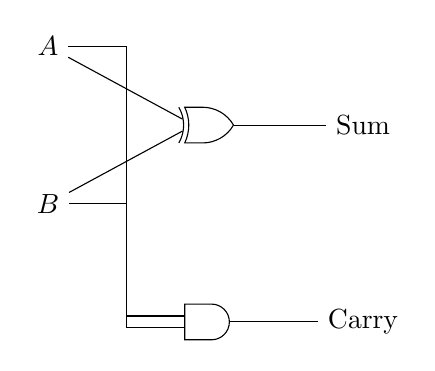
\begin{tikzpicture}[circuit logic US, scale=1, transform shape]

		% Inputs
		\node (A) at (0, 2) {\( A \)};
		\node (B) at (0, 0) {\( B \)};

		% XOR gate
		\node [xor gate US, draw, logic gate inputs=nn] (xor1) at (2, 1) {};
		\draw (A) -- (xor1.input 1);
		\draw (B) -- (xor1.input 2);

		% AND gate
		\node [and gate US, draw, logic gate inputs=nn] (and1) at (2, -1.5) {};
		\draw (A) -- ++(1,0) |- (and1.input 1);
		\draw (B) -- ++(1,0) |- (and1.input 2);

		% Outputs
		\node (Sum) at (4, 1) {\( \text{Sum} \)};
		\node (Carry) at (4, -1.5) {\( \text{Carry} \)};
		\draw (xor1.output) -- (Sum);
		\draw (and1.output) -- (Carry);

	\end{tikzpicture}
\end{center}

The XOR gate produces the sum bit, while the AND gate produces the carry bit. This forms the fundamental building block of a full binary adder.

\section{Adding Two Single-Byte Binary Numbers Using XOR and AND}

Binary addition can be performed on two single-byte numbers using bitwise operations. Specifically:
- The \textbf{XOR (Exclusive OR)} operation gives the sum of two bits without considering the carry.
- The \textbf{AND} operation identifies where a carry will occur.
- The carry is then shifted left by one position and added to the result in subsequent iterations.

\textbf{Algorithm:}
1. Compute the sum without carry using XOR:
\[
	\text{sum} = a \oplus b
\]
2. Compute the carry using AND and shift it left by one bit:
\[
	\text{carry} = (a \land b) \ll 1
\]
3. Repeat the process by adding the carry to the sum until there is no carry left.

\textbf{Diagram:}
Below is a diagram that illustrates the process for a single bit addition.

\begin{center}
	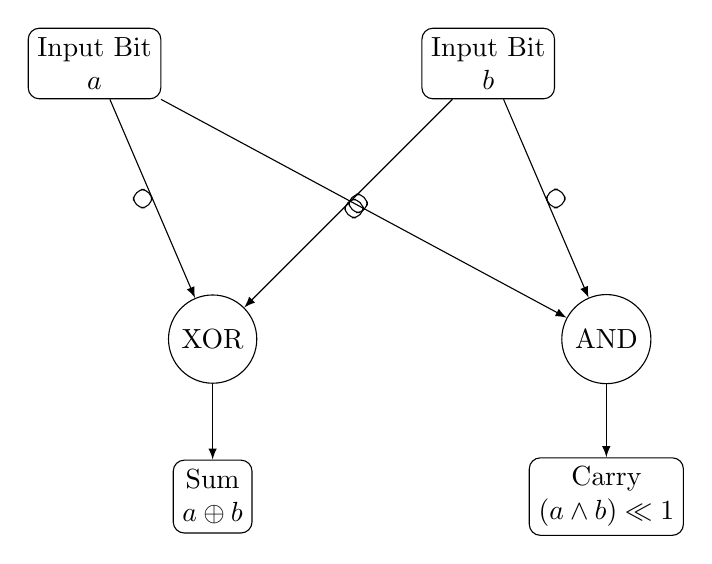
\begin{tikzpicture}[node distance=2cm, every node/.style={draw, rectangle, rounded corners, align=center}]
		% Nodes
		\node (A) {Input Bit \\ $a$};
		\node (B) [right of=A, xshift=3cm] {Input Bit \\ $b$};
		\node (XOR) [below of=A, yshift=-1.5cm, xshift=1.5cm, draw, circle] {XOR};
		\node (SUM) [below of=XOR] {Sum \\ $a \oplus b$};
		\node (AND) [right of=XOR, xshift=3cm, draw, circle] {AND};
		\node (CARRY) [below of=AND] {Carry \\ $(a \land b) \ll 1$};

		% Arrows
		\draw[->] (A) -- (XOR) node[midway, left] {};
		\draw[->] (B) -- (XOR) node[midway, right] {};
		\draw[->] (XOR) -- (SUM);
		\draw[->] (A) -- (AND) node[midway, left] {};
		\draw[->] (B) -- (AND) node[midway, right] {};
		\draw[->] (AND) -- (CARRY);
	\end{tikzpicture}
\end{center}

\textbf{Example:}
Consider two single-byte binary numbers:
\[
	a = 01101101, \quad b = 10101001
\]

1. Compute the XOR for the sum:
\[
	\text{sum} = a \oplus b = 11000100
\]

2. Compute the AND for the carry and shift left:
\[
	\text{carry} = (a \land b) \ll 1 = 00001010
\]

3. Add the sum and carry:
- New sum: \( \text{sum} = 11000100 \oplus 00001010 = 11001110 \)
- New carry: \( \text{carry} = (11000100 \land 00001010) \ll 1 = 00000000 \)

4. Final result: \( 11001110 \).

\section{One's Complement for a Single Byte}

The \textbf{one's complement} of a binary number is obtained by flipping all the bits, changing every \texttt{1} to \texttt{0} and every \texttt{0} to \texttt{1}. This operation is commonly used in binary arithmetic, particularly in representing negative numbers in early computing systems.

\textbf{Steps to Compute One's Complement:}
1. Write down the binary number.
2. Flip all bits:
- Change each \texttt{0} to \texttt{1}.
- Change each \texttt{1} to \texttt{0}.

\textbf{Example:}
Consider the binary number \(a = 01101101\).

1. Original binary number:
\[
	a = 01101101
\]

2. One's complement (flip all bits):
\[
	\text{one's complement of } a = 10010010
\]

\textbf{Diagram:}
The following diagram illustrates the transformation:

\begin{center}
	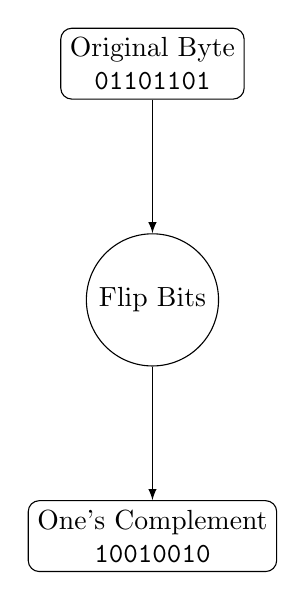
\begin{tikzpicture}[
			node distance=2cm,
			every node/.style={draw, rectangle, rounded corners, align=center}
		]
		% Nodes
		\node (Original) {Original Byte \\ \texttt{01101101}};
		\node (Flip) [below of=Original, yshift=-1cm, draw, circle] {Flip Bits};
		\node (Complement) [below of=Flip, yshift=-1cm] {One's Complement \\ \texttt{10010010}};

		% Arrows
		\draw[->] (Original) -- (Flip);
		\draw[->] (Flip) -- (Complement);
	\end{tikzpicture}
\end{center}

\textbf{Properties of One's Complement:}
- A binary number and its one's complement always sum to all \texttt{1}s (i.e., \(11111111\) for a single byte).
- One's complement is useful in representing signed integers:
- Positive numbers are represented as-is.
- Negative numbers are represented by the one's complement of their positive counterparts.

\textbf{Example with Signed Integers:}
For a single byte:
1. \(+5\) in binary: \(00000101\)
2. \(-5\) in one's complement: \(11111010\)

\textbf{Verification:}
Adding \(+5\) and \(-5\) in one's complement arithmetic:
\[
	00000101 + 11111010 = 11111111 \quad (\text{all bits are 1, representing zero in one's complement arithmetic}).
\]

\section{Carrying When Adding Negatives in One's Complement}

In one's complement representation, negative numbers are represented by flipping all the bits of their positive counterparts. When adding two negative numbers, a carry might be generated, which needs to be added back to the result to obtain the correct answer.

\textbf{Example:} Adding \(-3\) and \(-4\).

1. Represent \(-3\) and \(-4\) in one's complement for a single byte:
\[
	+3 = 00000011, \quad -3 = \text{one's complement of } +3 = 11111100
\]
\[
	+4 = 00000100, \quad -4 = \text{one's complement of } +4 = 11111011
\]

2. Add the two numbers:
\[
	\begin{array}{c@{}c@{}c@{}c@{}c@{}c@{}c@{}c@{}c}
		  & 1 & 1 & 1 & 1 & 1 & 1 & 0 & 0 \\
		+ & 1 & 1 & 1 & 1 & 1 & 0 & 1 & 1 \\ \hline
		  & 1 & 1 & 1 & 1 & 0 & 1 & 1 & 1 \\
	\end{array}
\]

3. Handle the carry:
- The result of the addition is \(11110111\), with a carry bit of \(1\).
- Add the carry back to the least significant bit:
\[
	11110111 + 1 = 11111000
\]

4. Final result:
\[
	11111000 = \text{one's complement of } +7 = -7
\]

\textbf{Explanation:}
- When the sum generates a carry, it must be added back to the result to comply with one's complement rules.
- The result of \(-3 + -4 = -7\), as expected.

\begin{center}
	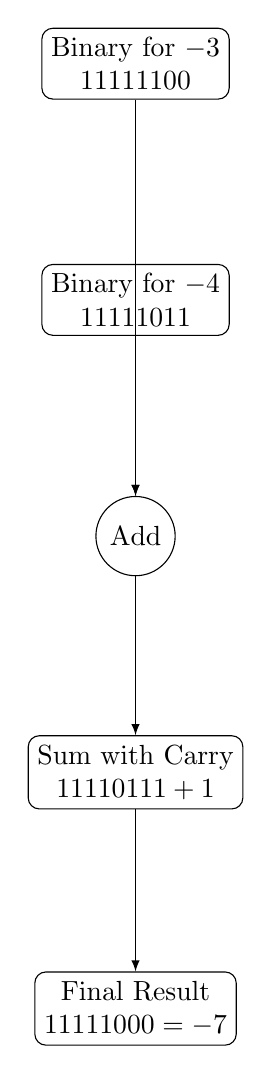
\begin{tikzpicture}[node distance=2cm, every node/.style={draw, rectangle, rounded corners, align=center}]
		% Nodes
		\node (A) {Binary for $-3$ \\ $11111100$};
		\node (B) [below of=A, yshift=-1cm] {Binary for $-4$ \\ $11111011$};
		\node (Add) [below of=B, yshift=-1cm, draw, circle] {Add};
		\node (Sum) [below of=Add, yshift=-1cm] {Sum with Carry \\ $11110111 + 1$};
		\node (Result) [below of=Sum, yshift=-1cm] {Final Result \\ $11111000 = -7$};

		% Arrows
		\draw[->] (A) -- (Add);
		\draw[->] (B) -- (Add);
		\draw[->] (Add) -- (Sum);
		\draw[->] (Sum) -- (Result);
	\end{tikzpicture}
\end{center}

\textbf{Note:} This approach works for signed integers in one's complement and highlights the importance of handling the carry bit to ensure accurate results.

\section{Two's Complement for a Single Byte}

The \textbf{two's complement} of a binary number is obtained by flipping all the bits (as in one's complement) and then adding \(1\) to the result. This method is widely used in modern computer systems to represent signed integers.

\textbf{Steps to Compute Two's Complement:}
1. Write down the binary number.
2. Flip all bits (as in one's complement).
3. Add \(1\) to the flipped number.

\textbf{Example:}
Consider the binary number \(a = 01101101\).

1. Original binary number:
\[
	a = 01101101
\]

2. Flip all bits (one's complement):
\[
	10010010
\]

3. Add \(1\) to the result:
\[
	\text{two's complement of } a = 10010010 + 1 = 10010011
\]

\textbf{Diagram:}
The following diagram illustrates the transformation:

\begin{center}
	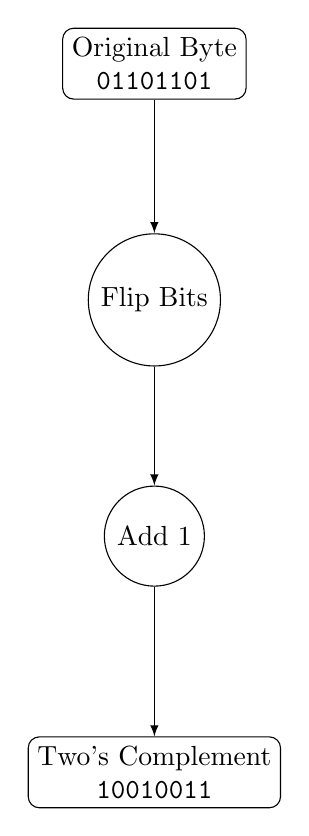
\begin{tikzpicture}[
			node distance=2cm,
			every node/.style={draw, rectangle, rounded corners, align=center}
		]
		% Nodes
		\node (Original) {Original Byte \\ \texttt{01101101}};
		\node (Flip) [below of=Original, yshift=-1cm, draw, circle] {Flip Bits};
		\node (Add) [below of=Flip, yshift=-1cm, draw, circle] {Add $1$};
		\node (Complement) [below of=Add, yshift=-1cm] {Two's Complement \\ \texttt{10010011}};

		% Arrows
		\draw[->] (Original) -- (Flip);
		\draw[->] (Flip) -- (Add);
		\draw[->] (Add) -- (Complement);
	\end{tikzpicture}
\end{center}

\textbf{Properties of Two's Complement:}
- The two's complement of \(0\) is \(0\), and the two's complement of the maximum negative value is itself.
- Negative numbers are represented by their two's complement.
- Addition and subtraction with two's complement do not require separate subtraction logic, simplifying arithmetic operations.

\section{Carrying When Adding Negatives in Two's Complement}

In two's complement representation, negative numbers are represented by flipping all bits of the positive number and adding \(1\). When adding two negative numbers, the carry generated during addition is discarded.

\textbf{Example:} Adding \(-3\) and \(-4\).

1. Represent \(-3\) and \(-4\) in two's complement for a single byte:
\[
	+3 = 00000011, \quad -3 = \text{two's complement of } +3 = 11111101
\]
\[
	+4 = 00000100, \quad -4 = \text{two's complement of } +4 = 11111100
\]

2. Add the two numbers:
\[
	\begin{array}{c@{}c@{}c@{}c@{}c@{}c@{}c@{}c@{}c}
		  & 1 & 1 & 1 & 1 & 1 & 1 & 1 & 0 \\
		+ & 1 & 1 & 1 & 1 & 1 & 1 & 0 & 0 \\ \hline
		  & 1 & 1 & 1 & 1 & 1 & 0 & 1 & 1 \\
	\end{array}
\]

3. Handle the carry:
- The result of the addition is \(11111011\).
- In two's complement, the carry is ignored, so the final result is:
\[
	11111011 = -7
\]

\textbf{Explanation:}
- In two's complement, the carry bit is discarded, unlike in one's complement.
- The result of \(-3 + -4 = -7\), as expected.

\begin{center}
	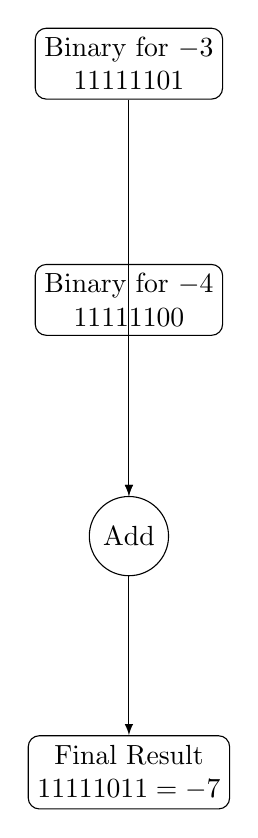
\begin{tikzpicture}[node distance=2cm, every node/.style={draw, rectangle, rounded corners, align=center}]
		% Nodes
		\node (A) {Binary for $-3$ \\ $11111101$};
		\node (B) [below of=A, yshift=-1cm] {Binary for $-4$ \\ $11111100$};
		\node (Add) [below of=B, yshift=-1cm, draw, circle] {Add};
		\node (Result) [below of=Add, yshift=-1cm] {Final Result \\ $11111011 = -7$};

		% Arrows
		\draw[->] (A) -- (Add);
		\draw[->] (B) -- (Add);
		\draw[->] (Add) -- (Result);
	\end{tikzpicture}
\end{center}

\textbf{Note:} Two's complement simplifies arithmetic operations by eliminating the need to add back the carry. It is the most commonly used method for representing signed integers in modern computing systems.

\chapter{Microarchitecture}

\section{Computer Architecture Overview}
\begin{tikzpicture}[
		>=Latex,            % arrow tip
		node distance=2.5cm,
		font=\small,
		align=center
	]

	%--- Processor, Memory, and I/O subsystem blocks
	\node[draw, minimum width=2.5cm, minimum height=3cm] (processor) {Processor};
	\node[draw, minimum width=2.5cm, minimum height=3cm, right=6cm of processor] (memory) {Memory};
	\node[draw, minimum width=2.5cm, minimum height=3cm, below=4cm of memory] (iosubsystem) {I/O Subsystem};

	%--- Buses between Processor and Memory
	% Address Bus
	\draw[->] (processor.east)++(0,0.8) --
	node[above]{\textbf{Address Bus}}
	($(memory.west)+(0,0.8)$);

	% Data Bus
	\draw[<->] (processor.east) --
	node[above]{\textbf{Data Bus}}
	(memory.west);

	% Control Bus
	\draw[->] (processor.east)++(0,-0.8) --
	node[above]{\textbf{Control Bus}}
	($(memory.west)+(0,-0.8)$);

	%--- Buses between Memory and I/O Subsystem
	% Address Bus
	\draw[->] ($(memory.south)+(0.6,0)$) --
	node[right, xshift=0.1cm]{\textbf{Address Bus}}
	($(iosubsystem.north)+(0.6,0)$);

	% Data Bus
	\draw[<->] (memory.south) --
	node[right]{\textbf{Data Bus}}
	(iosubsystem.north);

	% Control Bus
	\draw[->] ($(memory.south)+(-0.6,0)$) --
	node[right, xshift=-0.1cm]{\textbf{Control Bus}}
	($(iosubsystem.north)+(-0.6,0)$);

	%--- I/O Devices (circles off to the right, for example)
	\node[draw, circle, right=2cm of iosubsystem] (iodev1) {I/O\\device};
	\node[draw, circle, above=1.2cm of iodev1] (iodev2) {I/O\\device};
	\node[draw, circle, below=1.2cm of iodev1] (iodev3) {I/O\\device};

	\draw[->] (iosubsystem.east) -- (iodev1.west);
	\draw[->] (iosubsystem.east |- iodev2.west) -- (iodev2.west);
	\draw[->] (iosubsystem.east |- iodev3.west) -- (iodev3.west);

\end{tikzpicture}
\subsection{Address Bus}

The address bus is a critical component in a computer's architecture, responsible for specifying the memory addresses that the processor will read from or write to. The width of the address bus determines the maximum amount of memory that can be addressed by the system.

\textbf{Address Bus Width and Memory Capacity:}

- \textbf{8-bit Address Bus:}
- Can address \(2^8 = 256\) memory locations.
- Each memory location typically holds 1 byte of data.
- Total addressable memory: 256 bytes.

- \textbf{16-bit Address Bus:}
- Can address \(2^{16} = 65,536\) memory locations.
- Each memory location typically holds 1 byte of data.
- Total addressable memory: 65,536 bytes (or 64 KB).

- \textbf{32-bit Address Bus:}
- Can address \(2^{32} = 4,294,967,296\) memory locations.
- Each memory location typically holds 1 byte of data.
- Total addressable memory: 4,294,967,296 bytes (or 4 GB).

- \textbf{64-bit Address Bus:}
- Can address \(2^{64} = 18,446,744,073,709,551,616\) memory locations.
- Each memory location typically holds 1 byte of data.
- Total addressable memory: 18,446,744,073,709,551,616 bytes (or 16 exabytes).

\textbf{Example: 16-bit Address Bus}

For a 16-bit address bus, the number of unique addresses is calculated as follows:
\[
	2^{16} = 65,536 \text{ addresses}
\]
Each address corresponds to a unique memory cell, allowing the processor to access up to 65,536 different memory locations. If each memory location holds 1 byte, the total addressable memory is 65,536 bytes (or 64 KB).

\textbf{Diagram:}

\begin{center}
	\begin{tikzpicture}[
			>=Latex,            % arrow tip
			node distance=2.5cm,
			font=\small,
			align=center
		]

		%--- Processor and Memory blocks
		\node[draw, minimum width=2.5cm, minimum height=3cm] (processor) {Processor};
		\node[draw, minimum width=2.5cm, minimum height=3cm, right=6cm of processor] (memory) {Memory};

		%--- Address Bus
		\draw[->] (processor.east)++(0,0.8) --
		node[above]{\textbf{Address Bus (16-bit)}}
		($(memory.west)+(0,0.8)$);

		%--- Data Bus
		\draw[<->] (processor.east) --
		node[above]{\textbf{Data Bus}}
		(memory.west);

		%--- Control Bus
		\draw[->] (processor.east)++(0,-0.8) --
		node[above]{\textbf{Control Bus}}
		($(memory.west)+(0,-0.8)$);

	\end{tikzpicture}
\end{center}

The address bus plays a crucial role in determining the system's memory capacity and overall performance. A wider address bus allows for more memory to be accessed, which is essential for modern applications and operating systems.

\subsection{Data Bus}

The data bus is a bidirectional pathway that transfers data between the processor, memory, and I/O devices. It plays a crucial role in the fetch-execute cycle, enabling the processor to read instructions and data from memory and write results back to memory.

\textbf{Multidirectionality in the Fetch-Execute Cycle:}
1. \textbf{Fetch:} The processor uses the data bus to read an instruction from memory.
2. \textbf{Decode:} The instruction is decoded internally by the processor.
3. \textbf{Execute:} The processor may read or write data to/from memory or I/O devices using the data bus.

\textbf{Bandwidth and Cell Size:}
- The width of the data bus determines the amount of data transferred in one cycle.
- A wider data bus can transfer more data per cycle, increasing overall system performance.
- For example, a 32-bit data bus can transfer 4 bytes per cycle, while a 64-bit data bus can transfer 8 bytes per cycle.

\textbf{Example: 32-bit Data Bus}

For a 32-bit data bus, the amount of data transferred per cycle is calculated as follows:
\[
	\text{Data per cycle} = 32 \text{ bits} = 4 \text{ bytes}
\]

\textbf{Diagram:}

\begin{center}
	\begin{tikzpicture}[
			>=Latex,            % arrow tip
			node distance=2.5cm,
			font=\small,
			align=center
		]

		%--- Processor and Memory blocks
		\node[draw, minimum width=2.5cm, minimum height=3cm] (processor) {Processor};
		\node[draw, minimum width=2.5cm, minimum height=3cm, right=6cm of processor] (memory) {Memory};

		%--- Data Bus
		\draw[<->] (processor.east) --
		node[above]{\textbf{Data Bus (32-bit)}}
		(memory.west);

	\end{tikzpicture}
\end{center}

The data bus's bidirectional nature and bandwidth are critical for efficient data transfer, directly impacting the system's speed and performance.

\subsection{Processor Components}

The processor, also known as the Central Processing Unit (CPU), is the brain of the computer. It performs calculations, executes instructions, and manages data flow within the system. Key components of the processor include registers, the program counter (PC), and the EFLAGS register.

\subsubsection{Registers}

Registers are small, fast storage locations within the CPU used to hold data temporarily during execution. They are crucial for the processor's operation, allowing quick access to frequently used values. In this architecture, we have general-purpose registers and special-purpose registers.

\textbf{General-Purpose Registers:}
- The CPU has six general-purpose registers, named \(r0\) to \(r5\).
- Each register can store 16 bits of data.
- These registers are used for various operations, such as arithmetic, logic, and data manipulation.

\textbf{Example:}
\[
	\begin{array}{|c|c|}
		\hline
		\text{Register} & \text{Value (Binary)} \\
		\hline
		r0              & 0000000000000001      \\
		r1              & 0000000000000010      \\
		r2              & 0000000000000011      \\
		r3              & 0000000000000100      \\
		r4              & 0000000000000101      \\
		r5              & 0000000000000110      \\
		\hline
	\end{array}
\]

\subsubsection{Program Counter (PC)}

The Program Counter (PC) is a special-purpose register that holds the address of the next instruction to be executed. It plays a critical role in the fetch-execute cycle, ensuring the CPU processes instructions in the correct sequence.

\textbf{Functionality:}
- The PC is automatically incremented after each instruction fetch, pointing to the next instruction in memory.
- If a jump or branch instruction is executed, the PC is updated to the target address, altering the flow of execution.

\textbf{Example:}
\[
	\text{PC} = 0000000000001000 \quad (\text{Next instruction address})
\]

\subsubsection{EFLAGS Register}

The EFLAGS register is a special-purpose, read-only register that holds the results of recent operations. It contains several flags that provide information about the state of the CPU and the outcome of arithmetic and logical operations.

\textbf{Key Flags:}
- \textbf{Zero Flag (ZF):} Indicates whether the result of an operation is zero.
- Set to 1 if the result is zero.
- Set to 0 if the result is non-zero.

\textbf{Example:}
\[
	\text{EFLAGS} = \begin{array}{|c|c|c|c|c|c|c|c|c|c|c|c|c|c|c|c|}
		\hline
		\text{15} & \text{14} & \text{13} & \text{12} & \text{11} & \text{10} & \text{9} & \text{8} & \text{7} & \text{6} & \text{5} & \text{4} & \text{3} & \text{2} & \text{1} & \text{0}  \\
		\hline
		0         & 0         & 0         & 0         & 0         & 0         & 0        & 0        & 0        & 0        & 0        & 0        & 0        & 0        & 0        & \text{ZF} \\
		\hline
	\end{array}
\]

\textbf{Usage:}
- The Zero Flag is commonly used in conditional branching. For example, a jump instruction may depend on whether the Zero Flag is set, allowing the CPU to make decisions based on the results of previous operations.

\textbf{Diagram:}
\begin{center}
	\begin{tikzpicture}[
			>=Latex,            % arrow tip
			node distance=2.5cm,
			font=\small,
			align=center
		]

		%--- Processor block
		\node[draw, minimum width=2.5cm, minimum height=3cm] (processor) {Processor};

		%--- Registers
		\node[draw, below=1cm of processor, minimum width=2.5cm] (registers) {Registers\\(r0-r5)};
		\draw[->] (processor.south) -- (registers.north);

		%--- Program Counter
		\node[draw, left=2cm of processor, minimum width=2.5cm] (pc) {Program Counter\\(PC)};
		\draw[->] (processor.west) -- (pc.east);

		%--- EFLAGS
		\node[draw, right=2cm of processor, minimum width=2.5cm] (eflags) {EFLAGS\\(Zero Flag)};
		\draw[->] (processor.east) -- (eflags.west);

	\end{tikzpicture}
\end{center}

These components work together to enable the processor to execute instructions efficiently, manage data flow, and make decisions based on the results of operations.

\chapter{Instruction Set}
\begin{itemize}
	\item We will go over all of the instructions that we will cover
	      in this class by example, including their assembly code.
	\item We will then learn how to represent each instruction in binary,
	      so that the hardware can understand it.
	\item We will work with them in binary only to start.
	\item Later, when we get to the Assembly level, we will be able to
	      represent the instructions in more readable form.
\end{itemize}

\section{Assembly Pseudocode Conventions}

\begin{itemize}
	\item \(R_n\): register \(n\) (where \(n\) is 0 through 5)
	\item \(*R_n\): data in register \(n\)
	\item \([R_n]\): memory cell at the address stored in register \(n\)
	\item \(R_n \leftarrow x\): contents of register \(n\) are now \(x\)
\end{itemize}
\ex{Addition}{
	assembly:
	$$add R_n, R_m$$
	pseudocode:
	$$R_n \leftarrow * R_n + * R_m$$
}

\ex{Subtraction}{
	assembly:
	$$sub R_n, R_m$$
	pseudocode:
	$$R_n \leftarrow * R_n - * R_m$$
}

\ex{XOR}{
	assembly:
	$$xor R_n, R_m$$
	pseudocode:
	$$R_n \leftarrow * R_n ^ * R_m$$
}

\ex{Compare}{
	assembly:
	$$cmp R_n, R_m$$
	pseudocode:
	$$EFLAGS \leftarrow compare(* R_n - * R_m)$$
}

\ex{increment}{
	assembly:
	$$increment R_n$$
	pseudocode:
	$$R_n \leftarrow * R_n +1$$
}

\ex{Move: copy data from register $R_n$ into the absolute address in memory stored in $R_m$}{
	assembly:
	$$mov [R_n], R_m$$
	pseudocode:
	$$Mem[*R_n] \leftarrow * R_m$$
	Intuition for busses:
	The address bus carries the memory address from the processor to the memory. The data bus transfers the actual data between the processor and memory. The control bus carries control signals from the processor to coordinate the operations of the memory and I/O devices.
}

\ex{Move: copy data from the absolute address in memory stored in $R_m$ into register $R_n$}{
	assembly:
	$$mov R_n, [R_m]$$
	pseudocode:
	$$R_n \leftarrow Mem[*R_m]$$
	Intuition for busses:
	The address bus carries the memory address from the processor to the memory. The data bus transfers the actual data between the processor and memory. The control bus carries control signals from the processor to coordinate the operations of the memory and I/O devices.
}

\ex{Jump if equals}{
	assembly:
	$$jeq [R_n]$$
	pseudocode:
	$$if (ZF == 1) \text{ then } PC \leftarrow * R_n$$
	Intuition: read (jump to that address) $R_n$ if the zero flag is 1.
}

\ex{move num to $R_n$}{
	assembly:
	$$mov R_n, num$$
	pseudocode:
	$$R_n \leftarrow num$$
}
\qs{Starting Conditions and Execution Flow}{%
	Given the following initial program state and instructions:

	\begin{itemize}
		\item \(\text{PC} = 0010\)
		\item \(\text{Mem}[0010] = \texttt{mov R0, 1010}\)
		\item \(\text{Mem}[0011] = \texttt{mov R1, 0001}\)
		\item \(\text{Mem}[0100] = \texttt{mov R4, 0110}\)
		\item \(\text{Mem}[0101] = \texttt{mov R5, 1011}\)
		\item \(\text{Mem}[0110] = \texttt{inc R1}\)
		\item \(\text{Mem}[0111] = \texttt{cmp R0, R1}\)
		\item \(\text{Mem}[1000] = \texttt{je R5}\)
		\item \(\text{Mem}[1001] = \texttt{cmp R0, R0}\)
		\item \(\text{Mem}[1010] = \texttt{je R4}\)
		\item \(\text{Mem}[1011] = \texttt{halt}\)
	\end{itemize}

	Explain, step by step, how this program executes until \(\texttt{halt}\).%
}

\sol
Here is the execution walkthrough:

\begin{enumerate}
	\item \textbf{PC = 0010:}
	      \(\texttt{mov R0, 1010}\).
	      This loads \(\texttt{1010}\) (binary) into \(R_0\).
	      Then \(\text{PC}\leftarrow 0011\).

	\item \textbf{PC = 0011:}
	      \(\texttt{mov R1, 0001}\).
	      Loads \(\texttt{0001}\) into \(R_1\).
	      Then \(\text{PC}\leftarrow 0100\).

	\item \textbf{PC = 0100:}
	      \(\texttt{mov R4, 0110}\).
	      Loads \(\texttt{0110}\) into \(R_4\).
	      Then \(\text{PC}\leftarrow 0101\).

	\item \textbf{PC = 0101:}
	      \(\texttt{mov R5, 1011}\).
	      Loads \(\texttt{1011}\) into \(R_5\).
	      Then \(\text{PC}\leftarrow 0110\).

	\item \textbf{PC = 0110:}
	      \(\texttt{inc R1}\).
	      Increments \(R_1\) from \(\texttt{0001}\) to \(\texttt{0010}\).
	      Then \(\text{PC}\leftarrow 0111\).

	\item \textbf{PC = 0111:}
	      \(\texttt{cmp R0, R1}\).
	      Compares \(R_0\) (\(\texttt{1010}\)) with \(R_1\) (\(\texttt{0010}\)).
	      Since they differ, the zero/equal flag is cleared.
	      Then \(\text{PC}\leftarrow 1000\).

	\item \textbf{PC = 1000:}
	      \(\texttt{je R5}\) (jump if equal).
	      The zero flag is 0, so no jump occurs.
	      Then \(\text{PC}\leftarrow 1001\).

	\item \textbf{PC = 1001:}
	      \(\texttt{cmp R0, R0}\).
	      Compares \(R_0\) with itself, which sets the zero flag to 1.
	      Then \(\text{PC}\leftarrow 1010\).

	\item \textbf{PC = 1010:}
	      \(\texttt{je R4}\).
	      Because the zero flag is 1, we jump to the address stored in \(R_4\),
	      which is \(\texttt{0110}\).
	      So \(\text{PC}\leftarrow 0110\), looping back.

	\item The loop repeats from \(\texttt{inc R1}\) until eventually \(R_1\)
	      equals \(R_0\) (\(\texttt{1010}\)).
	      At that point, the compare (\(\texttt{cmp R0, R1}\)) sets the zero flag,
	      and \(\texttt{je R5}\) at \(\text{PC}=1000\) finally jumps to \(R_5 = \texttt{1011}\),
	      which contains the \(\texttt{halt}\) instruction.
\end{enumerate}

This mechanism effectively keeps incrementing \(R_1\) until it matches \(R_0\),
then halts.

\section{Instruction Encoding for 16-bit Memory Cells}

Have been talking about 16-bit memory cells. Thus, our instructions and their parameters need to be able to be described and differentiated in 16-bits.

\subsection*{Encoding Rules}
\begin{itemize}
	\item \textbf{Zero-argument instructions}
	      \begin{itemize}
		      \item \texttt{halt} (only one): \texttt{0000 0000 0000 0000}
	      \end{itemize}

	\item \textbf{Single-argument instructions}
	      \begin{itemize}
		      \item First two bits are always \texttt{11}.
		      \item Use the first five bits to encode the instruction.
		      \item Use the remaining eleven bits to represent the argument.
	      \end{itemize}

	\item \textbf{Two-argument instructions}
	      \begin{itemize}
		      \item Use the first four bits to encode the instruction.
		      \item Use the next six bits for the first argument.
		      \item Use the final six bits for the second argument.
	      \end{itemize}
\end{itemize}

\section{Assemble}

To assemble a program is to convert it from human-readable instructions to
their binary representations

\pagebreak
\begin{table}[h]
	\centering
	% Reduce font size if needed
	\small
	% The total width is \textwidth, and we want 5 columns:
	%  1) Instruction
	%  2) Binary Code
	%  3) Description
	%  4) Arguments
	%  5) Example
	%
	% 'X' columns will wrap automatically.  If you need certain columns
	% narrower, you can use a fixed width, e.g. p{2.5cm} or similar.

	\begin{tabularx}{\textwidth}{@{}l l X X X@{}}
		\toprule
		\textbf{Instruction} & \textbf{Binary Code}                                                                   & \textbf{Description} & \textbf{Arguments} & \textbf{Example} \\
		\midrule
		\texttt{halt}
		                     & \texttt{0000 0000 0000 0000}
		                     & halt execution
		                     & none
		                     & \texttt{0000 0000 0000 0000}
		\\

		\texttt{inc R\_n}
		                     & \texttt{1100 0}
		                     & register R\_n gets (contents of R\_n) + 1
		                     & 11-bit argument representing \emph{n}
		                     & \texttt{inc R3}                                                                                                                                       \\
		                     &
		                     &
		                     &
		                     & \texttt{1100 0000 0000 0011}
		\\

		\texttt{jmp num}
		                     & \texttt{1100 1}
		                     & jump to \emph{relative} address \emph{num} by adding \emph{num} to the program counter
		                     & 11-bit argument representing \emph{num}
		                     & \texttt{jmp 25}                                                                                                                                       \\
		                     &
		                     &
		                     &
		                     & \texttt{1100 1000 0001 1001}
		\\

		\texttt{jne num}
		                     & \texttt{1101 0}
		                     & jump to relative address \emph{num} if last \texttt{cmp} was unequal
		                     & 11-bit argument representing \emph{num}
		                     & \texttt{jne 13}                                                                                                                                       \\
		                     &
		                     &
		                     &
		                     & \texttt{1101 0000 0000 1101}
		\\

		\texttt{je [R\_n]}
		                     & \texttt{1101 1}
		                     & jump to \emph{absolute} address in R\_n if last \texttt{cmp} was equal
		                     & 11-bit argument representing \emph{n}
		                     & \texttt{je [R3]}                                                                                                                                      \\
		                     &
		                     &
		                     &
		                     & \texttt{1101 1000 0000 0011}
		\\

		\texttt{add R\_n, R\_m}
		                     & \texttt{0001}
		                     & R\_n gets (R\_n + R\_m)
		                     & Two 6-bit arguments (first = n, next = m)
		                     & \texttt{add R3, R5}                                                                                                                                   \\
		                     &
		                     &
		                     &
		                     & \texttt{0001 0000 1100 0101}
		\\

		\texttt{sub R\_n, R\_m}
		                     & \texttt{0010}
		                     & R\_n gets (R\_n - R\_m)
		                     & Two 6-bit arguments (first = n, next = m)
		                     & \texttt{sub R3, R2}                                                                                                                                   \\
		                     &
		                     &
		                     &
		                     & \texttt{0010 0010 0100 1000}
		\\

		\texttt{xor R\_n, R\_m}
		                     & \texttt{0011}
		                     & R\_n gets bitwise XOR of R\_n and R\_m
		                     & Two 6-bit arguments (first = n, next = m)
		                     & \texttt{xor R2, R3}                                                                                                                                   \\
		                     &
		                     &
		                     &
		                     & \texttt{0011 0000 1000 0011}
		\\

		\texttt{cmp R\_n, R\_m}
		                     & \texttt{0100}
		                     & compare R\_n and R\_m; set flags accordingly
		                     & Two 6-bit arguments (first = n, next = m)
		                     & \texttt{cmp R5, R3}                                                                                                                                   \\
		                     &
		                     &
		                     &
		                     & \texttt{0100 0001 1100 0011}
		\\

		\texttt{mov R\_n, num}
		                     & \texttt{0101}
		                     & R\_n gets the value \emph{num}
		                     & Two 6-bit arguments (first = n, next = m)
		                     & \texttt{mov R5, 61}                                                                                                                                   \\
		                     &
		                     &
		                     &
		                     & \texttt{0101 0001 1111 1101}
		\\

		\texttt{mov R\_n, R\_m}
		                     & \texttt{0110}
		                     & R\_n gets the contents of R\_m
		                     & Two 6-bit arguments (first = n, next = m)
		                     & \texttt{mov R3, R1}                                                                                                                                   \\
		                     &
		                     &
		                     &
		                     & \texttt{0110 0001 0100 0001}
		\\

		\texttt{mov [R\_n], R\_m}
		                     & \texttt{0111}
		                     & copy contents of R\_m to memory address stored in R\_n
		                     & Two 6-bit arguments (first = n, next = m)
		                     & \texttt{mov [R3], R1}                                                                                                                                 \\
		                     &
		                     &
		                     &
		                     & \texttt{0111 0001 0100 0001}
		\\

		\texttt{mov R\_n, [R\_m]}
		                     & \texttt{1000}
		                     & copy from memory address in R\_m to R\_n
		                     & Two 6-bit arguments (first = n, next = m)
		                     & \texttt{mov R3, [R1]}                                                                                                                                 \\
		                     &
		                     &
		                     &
		                     & \texttt{1000 0001 0100 0001}
		\\
		\bottomrule
	\end{tabularx}
	\caption{Summary of instructions, binary codes, and examples.}
	\label{tab:instructions}
\end{table}

\pagebreak


\section{Binary to Hexadecimal Conversion}

Converting binary numbers to hexadecimal is straightforward because each hexadecimal digit represents four binary digits (bits). Here are the steps:

\begin{enumerate}
	\item \textbf{Group the binary digits into sets of four}, starting from the right. Add leading zeros if necessary to make a complete set.
	\item \textbf{Convert each group of four binary digits to its hexadecimal equivalent} using the following table:

	      \begin{center}
		      \begin{tabular}{|c|c|}
			      \hline
			      Binary & Hexadecimal \\
			      \hline
			      0000   & 0           \\
			      0001   & 1           \\
			      0010   & 2           \\
			      0011   & 3           \\
			      0100   & 4           \\
			      0101   & 5           \\
			      0110   & 6           \\
			      0111   & 7           \\
			      1000   & 8           \\
			      1001   & 9           \\
			      1010   & A           \\
			      1011   & B           \\
			      1100   & C           \\
			      1101   & D           \\
			      1110   & E           \\
			      1111   & F           \\
			      \hline
		      \end{tabular}
	      \end{center}
\end{enumerate}

\textbf{Example:} Convert the binary number \(11010110\) to hexadecimal.

\begin{enumerate}
	\item Group the binary digits: \(1101\) \(0110\).
	\item Convert each group:
	      \[
		      1101 = D, \quad 0110 = 6
	      \]
	\item Combine the hexadecimal digits: \(D6\).
\end{enumerate}

Thus, \(11010110_2 = D6_{16}\).

\section{Machine Code Decoding}

\subsection{Hexadecimal Machine Code}
\begin{verbatim}
5000 504A 5094 7040 C000 4042 D7FC 0000
\end{verbatim}

\subsection{Instruction Breakdown}
\begin{itemize}
	\item \textbf{5000}
	      \begin{itemize}
		      \item Binary: 0101 0000 0000 0000
		      \item Instruction: \texttt{MOV R0, 0}
	      \end{itemize}

	\item \textbf{504A}
	      \begin{itemize}
		      \item Binary: 0101 0000 0100 1010
		      \item Instruction: \texttt{MOV R1, 10}
	      \end{itemize}

	\item \textbf{5094}
	      \begin{itemize}
		      \item Binary: 0101 0000 1001 0100
		      \item Instruction: \texttt{MOV R2, 20}
	      \end{itemize}

	\item \textbf{7040}
	      \begin{itemize}
		      \item Binary: 0111 0000 0100 0000
		      \item Instruction: \texttt{MOV [R1], R0}
	      \end{itemize}

	\item \textbf{C000}
	      \begin{itemize}
		      \item Binary: 1100 0000 0000 0000
		      \item Instruction: \texttt{INC R0}
	      \end{itemize}

	\item \textbf{C001}
	      \begin{itemize}
		      \item Binary: 1100 0000 0000 0001
		      \item Instruction: \texttt{INC R1}
	      \end{itemize}

	\item \textbf{4042}
	      \begin{itemize}
		      \item Binary: 0100 0000 0100 0010
		      \item Instruction: \texttt{CMP R1, R2}
	      \end{itemize}

	\item \textbf{D7FC}
	      \begin{itemize}
		      \item Binary: 1101 0111 1111 1100
		      \item Instruction: \texttt{JNE -4}
	      \end{itemize}

	\item \textbf{0000}
	      \begin{itemize}
		      \item Binary: 0000 0000 0000 0000
		      \item Instruction: \texttt{HALT}
	      \end{itemize}
\end{itemize}

\subsection{Program Behavior}
\begin{enumerate}
	\item \texttt{MOV R0, 0} sets register \texttt{R0} to 0.
	\item \texttt{MOV R1, 10} sets register \texttt{R1} to 10.
	\item \texttt{MOV R2, 20} sets register \texttt{R2} to 20.
	\item \texttt{MOV [R1], R0} writes the contents of \texttt{R0} into memory at the address held by \texttt{R1}.
	\item \texttt{INC R0} increments \texttt{R0}.
	\item \texttt{INC R1} increments \texttt{R1}.
	\item \texttt{CMP R1, R2} compares \texttt{R1} and \texttt{R2}.
	\item \texttt{JNE -4} jumps back 4 instructions if \texttt{R1} is not equal to \texttt{R2}.
	\item \texttt{HALT} ends execution.
\end{enumerate}

\paragraph{Summary:}
This program uses a loop to:
\begin{itemize}
	\item Increment \texttt{R0} and \texttt{R1}
	\item Store \texttt{R0}’s value at memory address \texttt{R1}
	\item Stop once \texttt{R1} reaches \texttt{R2} (i.e., 20)
\end{itemize}
In effect, it writes an increasing sequence of values (0,\,1,\,2,\,$\ldots$) into consecutive memory locations starting at address 10, and halts once it has written the value 9 at address 19 (because at that point \texttt{R1} becomes 20, matching \texttt{R2}, so the loop ends).

\section{Fetch-Decode-Execute-Store Cycle}

The fetch-decode-execute-store cycle is the fundamental process by which a computer executes instructions. This cycle involves several key components: the Program Counter (PC), Instruction Register (IR), and various other registers and buses.

\subsection{Fetch}

1. The PC holds the address of the next instruction to be executed.
2. The address is sent to memory via the address bus.
3. The instruction at that address is fetched from memory and loaded into the IR.

\subsection{Decode}

1. The control unit reads the instruction in the IR.
2. The instruction is decoded to determine the operation to be performed and the operands involved.

\subsection{Execute}

1. The control unit signals the appropriate components (ALU, registers, etc.) to perform the operation.
2. The ALU or other execution units carry out the operation using the operands.

\subsection{Store}

1. The result of the operation is stored in the appropriate location (register or memory).
2. The PC is updated to point to the next instruction, and the cycle repeats.

\textbf{Diagram:}

\begin{center}
	\begin{tikzpicture}[
			>=Latex,            % arrow tip
			node distance=2.5cm,
			font=\small,
			align=center
		]

		%--- Processor block
		\node[draw, minimum width=2.5cm, minimum height=3cm] (processor) {Processor};

		%--- Program Counter
		\node[draw, left=2cm of processor, minimum width=2.5cm] (pc) {Program Counter\\(PC)};
		\draw[->] (processor.west) -- (pc.east);

		%--- Instruction Register
		\node[draw, right=2cm of processor, minimum width=2.5cm] (ir) {Instruction Register\\(IR)};
		\draw[->] (processor.east) -- (ir.west);

		%--- Memory
		\node[draw, below=2cm of processor, minimum width=2.5cm] (memory) {Memory};
		\draw[->] (processor.south) -- (memory.north);

		%--- Control Unit
		\node[draw, above=2cm of processor, minimum width=2.5cm] (control) {Control Unit};
		\draw[->] (processor.north) -- (control.south);

	\end{tikzpicture}
\end{center}

This cycle ensures that instructions are processed sequentially and efficiently, allowing the computer to perform complex tasks by breaking them down into simpler operations.

\section{Five-Stage Pipeline for Operations}

The five-stage pipeline is a common technique used in computer architecture to improve instruction throughput. Each instruction passes through five distinct stages: Fetch, Decode, Execute, Memory Access, and Write Back. Below are the details of each stage:

\subsection{1. Fetch (IF)}

\textbf{Instruction Fetch:}
- The instruction is fetched from memory.
- The Program Counter (PC) holds the address of the instruction to be fetched.
- The fetched instruction is stored in the Instruction Register (IR).

\textbf{Key Points:}
- The PC is incremented to point to the next instruction.
- This stage involves reading from memory, which can introduce delays if the memory access time is significant.

\subsection{2. Decode (ID)}

\textbf{Instruction Decode:}
- The fetched instruction is decoded to determine the operation and the operands.
- The control unit generates the necessary control signals based on the decoded instruction.
- The source operands are read from the register file.

\textbf{Key Points:}
- This stage involves interpreting the binary instruction and preparing the necessary data for execution.
- The control signals generated will guide the subsequent stages.

\subsection{3. Execute (EX)}

\textbf{Execution:}
- The actual operation specified by the instruction is performed.
- This could involve arithmetic or logical operations performed by the Arithmetic Logic Unit (ALU).
- For branch instructions, the target address is calculated.

\textbf{Key Points:}
- The ALU performs the required computation.
- The result of the computation is temporarily stored for the next stage.

\subsection{4. Memory Access (MEM)}

\textbf{Memory Access:}
- If the instruction involves memory access (e.g., load or store), the memory address is accessed.
- For load instructions, data is read from memory and stored in a temporary register.
- For store instructions, data is written to the specified memory address.

\textbf{Key Points:}
- This stage is crucial for instructions that interact with memory.
- Memory access can introduce delays due to varying memory access times.

\subsection{5. Write Back (WB)}

\textbf{Write Back:}
- The result of the instruction is written back to the register file.
- This updates the destination register with the computed value or the data read from memory.

\textbf{Key Points:}
- This stage ensures that the results of the instruction are stored for future use.
- The pipeline is now ready to process the next instruction.

\textbf{Diagram:}

\begin{center}
	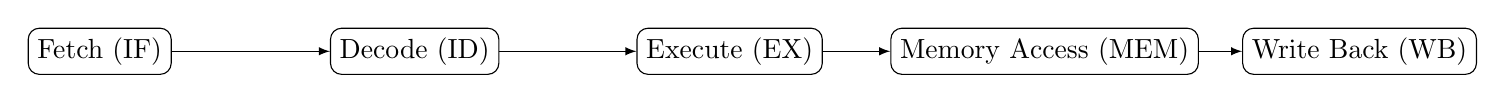
\begin{tikzpicture}[
			node distance=2cm,
			every node/.style={draw, rectangle, rounded corners, align=center}
		]

		% Nodes for each stage
		\node (IF) {Fetch (IF)};
		\node (ID) [right of=IF, xshift=2cm] {Decode (ID)};
		\node (EX) [right of=ID, xshift=2cm] {Execute (EX)};
		\node (MEM) [right of=EX, xshift=2cm] {Memory Access (MEM)};
		\node (WB) [right of=MEM, xshift=2cm] {Write Back (WB)};

		% Arrows between stages
		\draw[->] (IF) -- (ID);
		\draw[->] (ID) -- (EX);
		\draw[->] (EX) -- (MEM);
		\draw[->] (MEM) -- (WB);

	\end{tikzpicture}
\end{center}

The five-stage pipeline allows for overlapping execution of multiple instructions, significantly improving the instruction throughput and overall performance of the processor.

\begin{figure}[h]
	\centering
	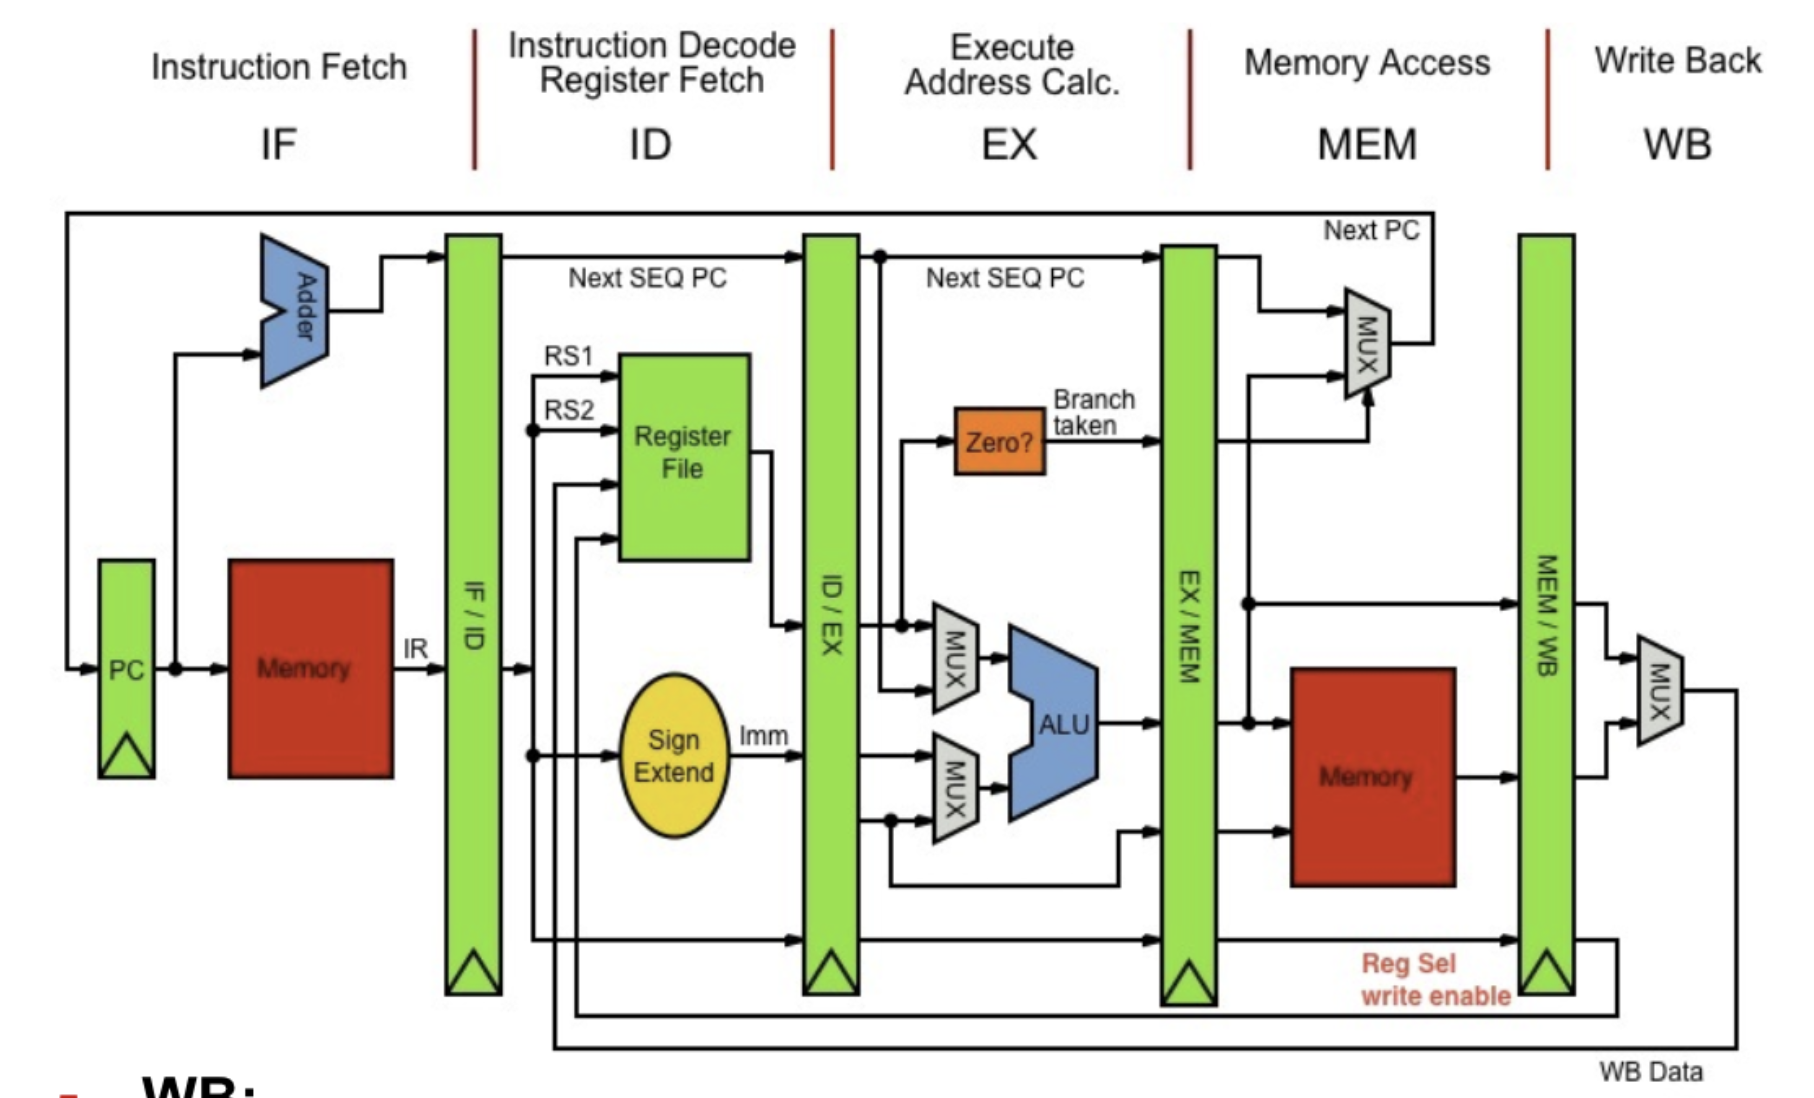
\includegraphics[width=\textwidth]{5stage.png}
	\caption{Five-Stage Pipeline for Operations}
	\label{fig:5stage}
\end{figure}

\subsection{Example of parallel processing in 5 stage pipeline}

\begin{table}[h!]
	\centering
	\begin{tabularx}{\textwidth}{@{}l*{5}{>{\centering\arraybackslash}X}@{}}
		\toprule
		\textbf{Cycle} & \textbf{IF} & \textbf{ID} & \textbf{EX} & \textbf{MEM} & \textbf{WB} \\
		\midrule
		1              & MOV R1 [R2] &             &             &              &             \\
		2              & ADD R3 R4   & MOV R1 [R2] &             &              &             \\
		3              & MOV [R5] R6 & ADD R3 R4   & MOV R1 [R2] &              &             \\
		4              &             & MOV [R5] R6 & ADD R3 R4   & MOV R1 [R2]  &             \\
		5              &             &             & MOV [R5] R6 & ADD R3 R4    & MOV R1 [R2] \\
		6              &             &             &             & MOV [R5] R6  & ADD R3 R4   \\
		7              &             &             &             &              & MOV [R5] R6 \\
		\bottomrule
	\end{tabularx}
	\caption{Pipeline Execution Table}
\end{table}

\section{Stalling and Forwarding in a 5-Stage Pipeline}

In a 5-stage pipeline, conflicts can arise when instructions that depend on the results of previous instructions are executed concurrently. Two common methods to overcome these conflicts are stalling and forwarding.

\subsection{Stalling}

Stalling, also known as pipeline interlock, involves pausing the pipeline until the data required by an instruction is available. This method ensures that instructions are executed in the correct order, but it can reduce the overall performance due to idle cycles.

\textbf{Example:}
Consider the following sequence of instructions:
\begin{verbatim}
1. MOV R1, [R2]
2. ADD R3, R1
\end{verbatim}

In this case, the ADD instruction depends on the result of the MOV instruction. To resolve this conflict, the pipeline can be stalled until the MOV instruction completes.

\textbf{Diagram:}
\begin{center}
	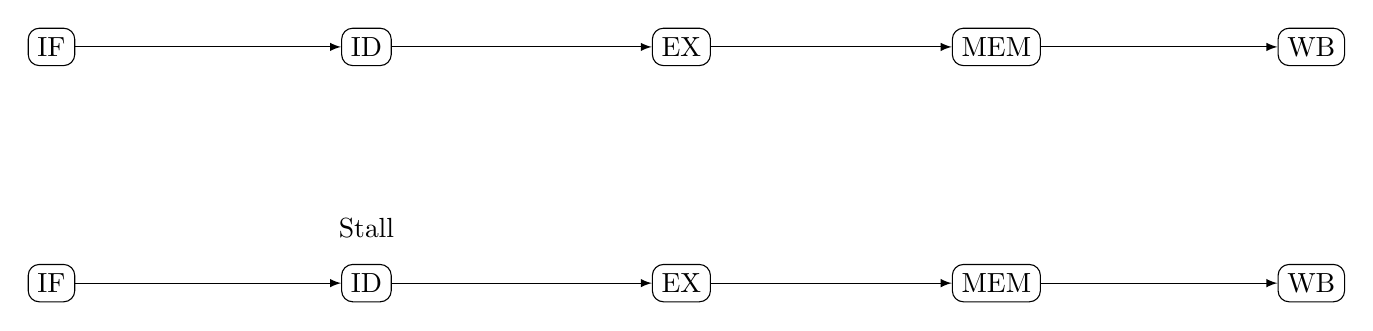
\begin{tikzpicture}[
			node distance=2cm,
			every node/.style={draw, rectangle, rounded corners, align=center}
		]

		% Nodes for each stage
		\node (IF1) {IF};
		\node (ID1) [right of=IF1, xshift=2cm] {ID};
		\node (EX1) [right of=ID1, xshift=2cm] {EX};
		\node (MEM1) [right of=EX1, xshift=2cm] {MEM};
		\node (WB1) [right of=MEM1, xshift=2cm] {WB};

		\node (IF2) [below of=IF1, yshift=-1cm] {IF};
		\node (ID2) [right of=IF2, xshift=2cm] {ID};
		\node (EX2) [right of=ID2, xshift=2cm] {EX};
		\node (MEM2) [right of=EX2, xshift=2cm] {MEM};
		\node (WB2) [right of=MEM2, xshift=2cm] {WB};

		% Arrows between stages
		\draw[->] (IF1) -- (ID1);
		\draw[->] (ID1) -- (EX1);
		\draw[->] (EX1) -- (MEM1);
		\draw[->] (MEM1) -- (WB1);

		\draw[->] (IF2) -- (ID2);
		\draw[->] (ID2) -- (EX2);
		\draw[->] (EX2) -- (MEM2);
		\draw[->] (MEM2) -- (WB2);

		% Stalling
		\node[draw=none, yshift=20px] at (ID2) {Stall};

	\end{tikzpicture}
\end{center}

\subsection{Forwarding}

Forwarding, also known as bypassing, involves passing the result of an instruction directly to a subsequent instruction that needs it, without waiting for it to be written back to the register file. This method reduces the number of idle cycles and improves performance.

\textbf{Example:}
Consider the following sequence of instructions:
\begin{verbatim}
1. MOV R1, [R2]
2. ADD R3, R1
\end{verbatim}

In this case, the result of the MOV instruction can be forwarded directly to the ADD instruction, allowing it to proceed without stalling.

\textbf{Diagram:}
\begin{center}
	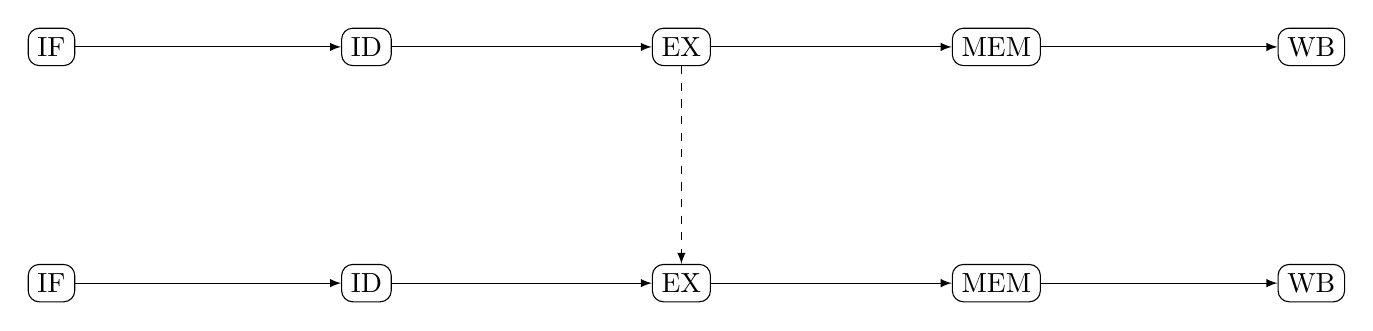
\begin{tikzpicture}[
			node distance=2cm,
			every node/.style={draw, rectangle, rounded corners, align=center}
		]

		% Nodes for each stage
		\node (IF1) {IF};
		\node (ID1) [right of=IF1, xshift=2cm] {ID};
		\node (EX1) [right of=ID1, xshift=2cm] {EX};
		\node (MEM1) [right of=EX1, xshift=2cm] {MEM};
		\node (WB1) [right of=MEM1, xshift=2cm] {WB};

		\node (IF2) [below of=IF1, yshift=-1cm] {IF};
		\node (ID2) [right of=IF2, xshift=2cm] {ID};
		\node (EX2) [right of=ID2, xshift=2cm] {EX};
		\node (MEM2) [right of=EX2, xshift=2cm] {MEM};
		\node (WB2) [right of=MEM2, xshift=2cm] {WB};

		% Arrows between stages
		\draw[->] (IF1) -- (ID1);
		\draw[->] (ID1) -- (EX1);
		\draw[->] (EX1) -- (MEM1);
		\draw[->] (MEM1) -- (WB1);

		\draw[->] (IF2) -- (ID2);
		\draw[->] (ID2) -- (EX2);
		\draw[->] (EX2) -- (MEM2);
		\draw[->] (MEM2) -- (WB2);

		% Forwarding
		\draw[->, dashed] (EX1) -- (EX2);

	\end{tikzpicture}
\end{center}

By using stalling and forwarding, the pipeline can handle data hazards and ensure correct execution of instructions while maintaining high performance.

\section{Handling Simultaneous Memory Reads in IF and WB Stages}

In a pipelined processor, simultaneous memory reads in the Instruction Fetch (IF) and Write Back (WB) stages can lead to conflicts and performance degradation. Two common approaches to address this issue are stalling and using the Harvard architecture.

\subsection{Stalling}

Stalling involves pausing the pipeline to resolve memory access conflicts. When a memory read conflict is detected, the pipeline is stalled until the memory access is completed. This ensures that the correct data is read, but it can reduce overall performance due to idle cycles.

\textbf{Example:}
Consider the following sequence of instructions:
\begin{verbatim}
1. MOV R1, [R2]
2. ADD R3, R1
\end{verbatim}

If both instructions require memory access at the same time, the pipeline can be stalled to resolve the conflict.

\textbf{Diagram:}
\begin{center}
	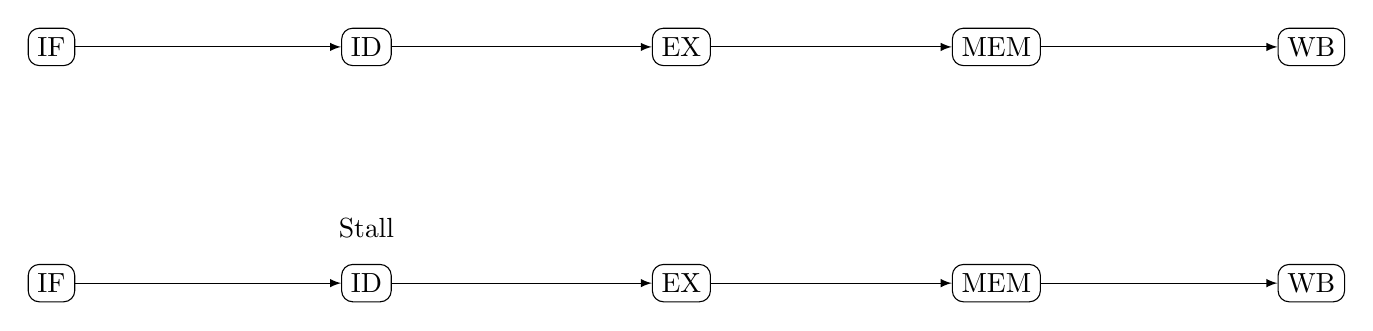
\begin{tikzpicture}[
			node distance=2cm,
			every node/.style={draw, rectangle, rounded corners, align=center}
		]

		% Nodes for each stage
		\node (IF1) {IF};
		\node (ID1) [right of=IF1, xshift=2cm] {ID};
		\node (EX1) [right of=ID1, xshift=2cm] {EX};
		\node (MEM1) [right of=EX1, xshift=2cm] {MEM};
		\node (WB1) [right of=MEM1, xshift=2cm] {WB};

		\node (IF2) [below of=IF1, yshift=-1cm] {IF};
		\node (ID2) [right of=IF2, xshift=2cm] {ID};
		\node (EX2) [right of=ID2, xshift=2cm] {EX};
		\node (MEM2) [right of=EX2, xshift=2cm] {MEM};
		\node (WB2) [right of=MEM2, xshift=2cm] {WB};

		% Arrows between stages
		\draw[->] (IF1) -- (ID1);
		\draw[->] (ID1) -- (EX1);
		\draw[->] (EX1) -- (MEM1);
		\draw[->] (MEM1) -- (WB1);

		\draw[->] (IF2) -- (ID2);
		\draw[->] (ID2) -- (EX2);
		\draw[->] (EX2) -- (MEM2);
		\draw[->] (MEM2) -- (WB2);

		% Stalling
		\node[draw=none, yshift=20px] at (ID2) {Stall};

	\end{tikzpicture}
\end{center}

\subsection{Harvard Architecture}

The Harvard architecture addresses memory access conflicts by using separate memory spaces for instructions and data. This allows simultaneous access to both instruction and data memory, eliminating conflicts and improving performance.

\textbf{Example:}
In the Harvard architecture, the instruction memory and data memory are accessed independently, allowing the IF stage to fetch instructions while the WB stage writes data.

\textbf{Diagram:}
\begin{center}
	\begin{tikzpicture}[
			node distance=2cm,
			every node/.style={draw, rectangle, rounded corners, align=center}
		]

		% Nodes for each stage
		\node (IF) {IF};
		\node (ID) [right of=IF, xshift=2cm] {ID};
		\node (EX) [right of=ID, xshift=2cm] {EX};
		\node (MEM) [right of=EX, xshift=2cm] {MEM};
		\node (WB) [right of=MEM, xshift=2cm] {WB};

		% Instruction Memory
		\node (IMEM) [above of=IF, yshift=1cm] {Instruction Memory};
		\draw[->] (IMEM) -- (IF);

		% Data Memory
		\node (DMEM) [below of=MEM, yshift=-1cm] {Data Memory};
		\draw[->] (MEM) -- (DMEM);
		\draw[->] (DMEM) -- (WB);

		% Arrows between stages
		\draw[->] (IF) -- (ID);
		\draw[->] (ID) -- (EX);
		\draw[->] (EX) -- (MEM);
		\draw[->] (MEM) -- (WB);

	\end{tikzpicture}
\end{center}

By using separate memory spaces for instructions and data, the Harvard architecture allows for more efficient memory access and reduces the need for stalling, leading to improved overall performance.

\section{Memory Pointers}

\begin{itemize}[left=0pt]
	\item When we get into C (and C++ later), we will talk a \textbf{lot} about memory indirection (pointers).
	\item But you have already been exposed to the concept with our minimal Instruction Set!
	\item \textbf{What is memory indirection??}
	\item Which one feels like memory indirection?
	      \begin{itemize}
		      \item \texttt{MOV R1 [0x27]}
		      \item \texttt{MOV R1 [R2]}
	      \end{itemize}
	\item In the first case, we are reading an absolute memory address into \texttt{register-1}.
	\item In the second case, we are reading the memory address specified by the value of \texttt{register-2} into \texttt{register-1}.
	\item \textbf{The second case is memory indirection, and \texttt{register-2} is acting as a pointer!}
\end{itemize}
\section{Memory Indirection in C++}

\begin{verbatim}
int numbers[] = {10, 20, 30, 40, 50};
int size = sizeof(numbers) / sizeof(numbers[0]);
// Pointer to the first element of the array
int *ptr = numbers;
for (int i = 0; i < size; i++) {
	printf("Element %d: %d\n", i, *(ptr + i));
}
\end{verbatim}

\textbf{Explanation:}

This code demonstrates memory indirection using pointers in C. Here's a breakdown of how it works:

1. \texttt{int numbers[] = \{10, 20, 30, 40, 50\};}
- An array of integers is declared and initialized with values.

2. \texttt{int size = sizeof(numbers) / sizeof(numbers[0]);}
- The size of the array is calculated by dividing the total size of the array by the size of one element.

3. \texttt{int *ptr = numbers;}
- A pointer \texttt{ptr} is declared and initialized to point to the first element of the array.

4. \texttt{for (int i = 0; i < size; i++) \{}
- A loop is used to iterate through the array elements.

5. The value of each element is accessed using the pointer \texttt{ptr} with memory indirection (\texttt{*(ptr + i)}) and printed.

\textbf{Memory Indirection:}
- The expression \texttt{*(ptr + i)} uses memory indirection to access the value at the memory address pointed to by \texttt{ptr} plus \texttt{i}.
- This allows accessing array elements using pointer arithmetic, demonstrating how pointers can be used to indirectly access memory locations.

\chapter{OS and Assembly}

\section{Why is an OS needed}

\section{Why is an OS needed}

An operating system (OS) is essential for several reasons:

1. \textbf{Resource Management:}
- The OS manages hardware resources such as CPU, memory, and I/O devices, ensuring efficient and fair allocation among multiple programs.

2. \textbf{Program Execution:}
- The OS provides an environment for executing programs, handling tasks such as loading programs into memory, scheduling CPU time, and managing program execution.

3. \textbf{Memory Management:}
- The OS handles memory allocation and deallocation, ensuring that programs do not interfere with each other's memory space. This prevents issues such as memory corruption, where programs might write data into memory cells containing instructions, leading to unpredictable behavior and system crashes.

4. \textbf{File System Management:}
- The OS manages files and directories on storage devices, providing a structured way to store, retrieve, and organize data.

5. \textbf{Security and Access Control:}
- The OS enforces security policies, controlling access to system resources and protecting against unauthorized access and malicious activities.

6. \textbf{Error Handling:}
- The OS detects and handles errors, providing mechanisms for recovering from hardware and software failures.

7. \textbf{User Interface:}
- The OS provides a user interface, such as a command-line interface (CLI) or graphical user interface (GUI), allowing users to interact with the system and perform tasks.

8. \textbf{Device Management:}
- The OS manages device drivers, facilitating communication between the system and peripheral devices such as printers, keyboards, and network adapters.

Overall, the OS acts as an intermediary between users, applications, and hardware, ensuring the smooth and efficient operation of the computer system.

\section{Memory Virtualization}

Memory virtualization is a technique used by operating systems to provide an abstraction of physical memory, allowing each process to have its own virtual address space. This improves security, isolation, and efficient use of memory. Here are the key concepts:

\begin{enumerate}
	\item \textbf{Virtual Address Space:}
	      - Each process is given a virtual address space, which is a contiguous range of addresses that the process can use.
	      - The virtual address space is mapped to physical memory by the OS.
	      \begin{itemize}
		      \item \textbf{Virtual Memory} allows the OS to use disk space as an extension of physical memory by assigning more memory to its programs than it has in RAM.
	      \end{itemize}

	\item \textbf{Page Tables:}
	      - The OS uses page tables to keep track of the mapping between virtual addresses and physical addresses.
	      - Each entry in the page table corresponds to a page (a fixed-size block of memory) and contains the physical address of the page.

	\item \textbf{Paging:}
	      - Memory is divided into fixed-size pages (e.g., 4 KB).
	      - Virtual memory is also divided into pages of the same size.
	      - When a process accesses a virtual address, the OS translates it to a physical address using the page table.

	\item \textbf{Page Faults:}
	      - If a process accesses a virtual address that is not currently mapped to physical memory, a page fault occurs.
	      - The OS handles the page fault by loading the required page from disk into physical memory and updating the page table.

	\item \textbf{Swapping:}
	      - When physical memory is full, the OS may swap out pages that are not currently in use to disk, freeing up physical memory for other pages.
	      - Swapped-out pages are stored in a swap space on disk and can be swapped back into physical memory when needed.

	\item \textbf{Protection:}
	      - Memory virtualization provides isolation between processes, preventing one process from accessing the memory of another process.
	      - The OS enforces access control by setting permissions on pages (e.g., read, write, execute).

	\item \textbf{Translation Lookaside Buffer (TLB):}
	      - The TLB is a cache used to speed up the translation of virtual addresses to physical addresses.
	      - It stores recent translations, reducing the need to access the page table for every memory access.

\end{enumerate}

\section{Context Switching}

Context switching is the process of saving and restoring the state of a CPU so that multiple processes can share the CPU effectively. Even if the number of cores that are available are
greater than the number of processes, context switching is still necessary to handle interrupts and system calls. Here are the key steps involved in context switching:

1. \textbf{Save the Context:}
- The OS saves the state of the currently running process, including the contents of registers, program counter, and other CPU state information.
- This state is stored in a data structure called the process control block (PCB).

2. \textbf{Update the Process State:}
- The OS updates the state of the currently running process to indicate that it is no longer running (e.g., changing its state to "waiting" or "ready").

3. \textbf{Select the Next Process:}
- The OS selects the next process to run based on a scheduling algorithm (e.g., round-robin, priority-based).
- The selected process's state is updated to indicate that it is now running.

4. \textbf{Restore the Context:}
- The OS restores the state of the selected process from its PCB, including the contents of registers and program counter.
- The CPU is now ready to execute the selected process.

\textbf{Diagram:}

\begin{center}
	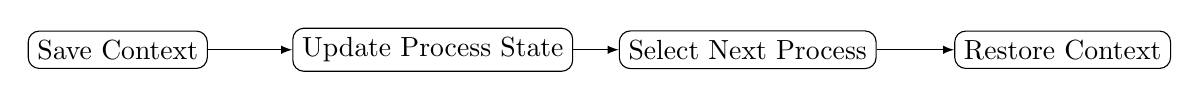
\begin{tikzpicture}[
			node distance=2cm,
			every node/.style={draw, rectangle, rounded corners, align=center}
		]

		% Nodes for each step
		\node (save) {Save Context};
		\node (update) [right of=save, xshift=2cm] {Update Process State};
		\node (select) [right of=update, xshift=2cm] {Select Next Process};
		\node (restore) [right of=select, xshift=2cm] {Restore Context};

		% Arrows between steps
		\draw[->] (save) -- (update);
		\draw[->] (update) -- (select);
		\draw[->] (select) -- (restore);

	\end{tikzpicture}
\end{center}

\chapter{C and C++}

\section{C Compilation}

\begin{itemize}
	\item \textbf{Preprocessing:}
	      \begin{itemize}
		      \item The preprocessor processes directives (e.g., \texttt{\#include}, \texttt{\#define}) and expands macros.
		      \item The output is a translation unit with all preprocessor directives processed.
	      \end{itemize}
	\item \textbf{Compilation:}
	      \begin{itemize}
		      \item The compiler translates the preprocessed source code into assembly code or object code.
		      \item The output is an object file containing machine code instructions.
	      \end{itemize}
	\item \textbf{Assembly:}
	      \begin{itemize}
		      \item The assembler translates the object code into machine code.
		      \item The output is an executable file that can be run on the target platform.
	      \end{itemize}
	\item \textbf{Linking:}
	      \begin{itemize}
		      \item The linker combines object files and libraries to create an executable file.
		      \item It resolves external references, assigns memory addresses, and generates the final executable.
	      \end{itemize}
	\item \textbf{Execution:}
	      \begin{itemize}
		      \item
		      \item The operating system loads the executable into memory and starts its execution.
	      \end{itemize}
\end{itemize}

\textbf{Compiled languages:} Translated to machine code before execution. \\
\textbf{Interpreted Languages:} Translated at runtime.

\subsection{Types and Casting}
\begin{verbatim}
	int c = a / b;
	printf("c is %d \n", c);
	\end{verbatim}

\ex{Integer Division Truncation}{
	Dividing two integers \texttt{a} (5) and \texttt{b} (2) results in truncation to an integer. The decimal part is discarded, leaving \texttt{c} with value 2.
}

\begin{verbatim}
	float d = 8 / 3;
	printf("d is %f \n", d);
	\end{verbatim}

\ex{Implicit Integer Division}{
	The expression \texttt{8/3} performs integer division first (resulting in 2), then assigns to float \texttt{d}. This demonstrates that division occurs before type conversion.
}

\begin{verbatim}
	float e = (float)a / b;
	printf("e is %f \n", e);
	\end{verbatim}

\ex{Explicit Casting for Floating-Point Division}{
	Casting \texttt{a} to \texttt{float} before division forces floating-point arithmetic. This produces a precise result (2.5) instead of truncation.
}

\dfn{Type Conversion in Division}{
	When at least one operand of the division operator (\texttt{/}) is a floating-point type, the result will be a floating-point value. Explicit casting can enforce this behavior.
}

\begin{verbatim}
	int g = a;
	printf("g is %d \n", g);
	\end{verbatim}

\nt{
	Assigning an integer to another integer preserves its value. This example appears redundant but demonstrates direct assignment between matching types.
}

\begin{verbatim}
	float h = int(f) / 2;
	printf("h is %f \n", h);
	\end{verbatim}

\ex{Double Truncation Example}{
	First truncates \texttt{f} (3.14159) to integer 3 via explicit cast, then performs integer division \texttt{3/2 = 1}. Finally assigns to float \texttt{h} as 1.0, showing two truncation steps.
}

\thm{Truncation Hierarchy}{
	Truncation occurs at each explicit cast or integer division operation. The order of operations determines whether decimal values are preserved or discarded.
}

\qs{Why does \texttt{h} equal 1.0?}{
	Explain why \texttt{int(f)/2} produces 1.0 instead of 1.5 when stored in a float.
}

\sol
The cast operation \texttt{int(f)} happens first, converting 3.14159 to integer 3. Then integer division \texttt{3/2} produces 1. Finally, this integer result is implicitly converted to float 1.0 during assignment to \texttt{h}.

\section{Fractions}

\dfn{Floating-Point Representation in C++}{
	In C++, floating-point numbers are represented according to the IEEE 754 standard. A single-precision (float) number consists of:
	\begin{itemize}
		\item \textbf{Sign bit (1 bit)}: Determines if the number is positive or negative.
		\item \textbf{Exponent (8 bits)}: Encodes the exponent in a biased format.
		\item \textbf{Mantissa (23 bits)}: Also known as the significand; represents the precision bits of the number.
	\end{itemize}
	The value of a floating-point number is computed as:
	\[
		(-1)^{\text{sign}} \times 2^{\text{exponent} - \text{bias}} \times (1 + \text{mantissa})
	\]
	For double-precision (double) numbers, the sizes differ (1 sign bit, 11 exponent bits, and 52 mantissa bits).
}

\nt{
	Floating-point arithmetic can introduce precision errors due to the finite number of bits used to represent real numbers. Operations that are mathematically exact might yield unexpected results in computer arithmetic.
}

\ex{Demonstration of Floating-Point Precision Loss}{
	Consider the following code that demonstrates the loss of precision when performing floating-point arithmetic:
}

\begin{verbatim}
void showFloatLossiness()
{
    double a = 0.1;
    double b = 0.2;
    double c = a + b;
    double d = c - b;
    printf("a: %.20f\n", a);
    printf("b: %.20f\n", b);
    printf("c: %.20f\n", c);
    printf("d: %.20f\n", d);
    printf("a == d: %s\n", a == d ? "true" : "false");
}
\end{verbatim}

When running this code, you might get the following output:

\begin{verbatim}
a: 0.10000000000000000555
b: 0.20000000000000001110
c: 0.30000000000000004441
d: 0.10000000000000000555
a == d: true
\end{verbatim}

This output shows that even simple arithmetic operations can result in floating-point numbers that have small differences from their expected values due to representation errors.


\nt{
	The loss of precision occurs because certain decimal fractions cannot be represented exactly in binary floating-point format. Numbers like 0.1 and 0.2 have infinite repeating binary representations, so they are approximated in a finite number of bits.
}

\dfn{Converting Decimal Fractions to Binary}{
	Converting a decimal fraction to binary involves multiplying the fractional part by 2 and recording the integer part at each step. This process repeats until the fractional part becomes zero or until a sufficient level of precision is achieved.
}

\ex{Example: Binary Representation of 12.5 as a Float}{
	Let's consider the decimal number 12.5 and examine its binary floating-point representation:

	\begin{enumerate}
		\item \textbf{Sign}: Positive, so the sign bit is 0.
		\item \textbf{Binary Form}: \(12.5_{10} = 1100.1_2\).
		\item \textbf{Normalized Form}: Shift the binary point to after the first 1: \(1.1001_2 \times 2^3\).
		\item \textbf{Exponent}: The exponent is \(3\). Adding the bias (127 for single-precision float): \(3 + 127 = 130\), which is \(10000010_2\) in binary.
		\item \textbf{Mantissa}: The mantissa is the fractional part after the leading 1: \(1001\), padded with zeros to fill 23 bits.
	\end{enumerate}

	Thus, the complete IEEE 754 binary representation is:

	\[
		\text{Sign bit}: 0 \quad \text{Exponent}: 10000010 \quad \text{Mantissa}: 10010000000000000000000
	\]
}

\nt{
	Due to limited precision, only a finite number of decimal fractions can be represented exactly in binary floating-point format. This limitation often leads to small rounding errors in calculations.
}

\ex{Converting a Decimal Number to a Binary Fraction in C++}{
	The following function converts a decimal number to its binary string representation, including the fractional part:
}

\begin{verbatim}
std::string convertToBinaryFraction(double num)
{
    // Check input bounds.
    if (num < 0)
    {
        return "Negative numbers not supported!";
    }
    if (num > 4294967295.0)
    {
        return "Input number too large!";
    }
    
    unsigned int intPart = static_cast<unsigned int>(num);
    double fracPart = num - intPart;
    
    // Convert integer part to binary.
    std::string intStr;
    if (intPart == 0)
    {
        intStr = "0";
    }
    else
    {
        while (intPart > 0)
        {
            intStr = std::to_string(intPart % 2) + intStr;
            intPart /= 2;
        }
    }
    
    // Convert fractional part to binary.
    std::string fracStr = ".";
    if (fracPart > 0)
    {
        int count = 0;
        while (fracPart > 0 && count < (32 - intStr.length()))
        {
            fracPart *= 2;
            if (fracPart >= 1)
            {
                fracStr += "1";
                fracPart -= 1;
            }
            else
            {
                fracStr += "0";
            }
            count++;
        }
    }
    else
    {
        fracStr += "0";
    }
    
    return intStr + fracStr;
}
\end{verbatim}

This function handles:
\begin{itemize}
	\item \textbf{Input validation}: Checks for negative numbers and excessively large inputs.
	\item \textbf{Integer part conversion}: Converts the integer part to binary by repeatedly dividing by 2.
	\item \textbf{Fractional part conversion}: Converts the fractional part to binary by multiplying by 2 and extracting the integer part.
	\item \textbf{Precision control}: Limits the number of iterations to prevent infinite loops with non-terminating binary fractions (e.g., \(1/3\)).
\end{itemize}


\nt{
	When converting fractions like \(1/3\) to binary, the fractional part does not terminate, resulting in infinite binary expansions. The function limits the precision based on the length of the integer part to mitigate excessive computation while providing a reasonable approximation.
}

\thm{Limitations of Binary Fraction Conversion}{
	Certain decimal fractions have infinite, non-repeating binary representations, similar to how \(1/3\) is infinite and non-repeating in decimal. Consequently, these numbers cannot be represented exactly in binary, leading to approximation errors in computations.
}

\section*{Types and Type Safety}

\begin{verbatim}
	unsigned int aa = 0x12345678;
	printf("Size of x is %zu bytes \n", sizeof(aa));
	\end{verbatim}

\dfn{Type Safety}{
	Degree to which a programming language prevents type errors. Contains two approaches:
	\begin{itemize}
		\item Weak typing: Flexible type interactions (may cause unexpected behaviors)
		\item Strong typing: Strict type enforcement (C++ uses this approach)
		      \begin{itemize}
			      \item Prevents operations between incompatible types
			      \item Enables better performance through optimized type handling
		      \end{itemize}
	\end{itemize}
}

\dfn{Type Checking}{
	Process of verifying type constraints. Two main approaches:
	\begin{itemize}
		\item Static checking (compile-time):
		      \begin{itemize}
			      \item Used in C++
			      \item Catches errors before execution
			      \item Enables optimizations
		      \end{itemize}
		\item Dynamic checking (runtime):
		      \begin{itemize}
			      \item Type verification during execution
			      \item Adds runtime overhead
		      \end{itemize}
	\end{itemize}
}

\begin{verbatim}
	int x = 2;
	double y = 3.5;
	double result = x + y;
	printf("Result is %f \n", result);
	\end{verbatim}

\ex{Implicit Type Conversion}{
	Demonstrates C++'s lenient type safety through \textit{arithmetic conversions}:
	\begin{itemize}
		\item \texttt{int x} promoted to \texttt{double} before addition
		\item Conversion hierarchy: \texttt{int}
		      →
		      → \texttt{double}
		\item Result maintains highest precision type (\texttt{double})
	\end{itemize}
}

\begin{verbatim}
	int a = -1;
	unsigned int b = 1;
	if (a < b) {
	printf("a is less than b \n");
	} else {
	printf("a is not less than b \n");
	}
	\end{verbatim}

\ex{Unsigned Conversion Pitfall}{
	Illustrates unexpected behavior with signed/unsigned comparisons:
	\begin{itemize}
		\item \texttt{int a} converted to \texttt{unsigned int} via \textit{integral promotions}
		\item -1 becomes 4294967295 (assuming 4-byte int)
		\item Comparison 4294967295 < 1 evaluates false
	\end{itemize}
}

\thm{Conversion Hierarchy Rule}{
	When operands have different types, the compiler will:
	\begin{enumerate}
		\item Promote smaller types to larger equivalents (\texttt{char}
		      →
		      → \texttt{int})
		\item Convert signed to unsigned if unsigned operand present
		\item Convert to floating-point if either operand is floating-point
	\end{enumerate}
}

\begin{verbatim}
	bool c = x < y;
	printf(c ? "true" : "false");
	\end{verbatim}

\nt{
	C++ allows comparisons between different arithmetic types:
	\begin{itemize}
		\item Compiler performs implicit conversions before comparison
		\item Conversion follows same hierarchy as arithmetic operations
		\item Result always \texttt{bool} type regardless of operand types
	\end{itemize}
}

\qs{Why does -1 appear larger than 1?}{
	Explain the counterintuitive result in the signed/unsigned comparison example.
}

\sol
The comparison converts both operands to unsigned integers. The signed value -1 becomes $2^{32}-1$
(maximum unsigned int value) in two's complement systems, making it numerically larger than 1. Always use explicit casts when comparing signed and unsigned values.

\section{Pointers}

\begin{verbatim}
	int square(int n) {
	int result = n * n;
	return result;
	}
	// ... other function definitions ...
	int exampleCallStack() {
	int a = 3, b = 4, c = 5;
	int result = sumOfSquares(a, b, c);
	std::cout << result << std::endl;
	return 0;
	}
\end{verbatim}

\dfn{Memory Segments in C++}{
	Program memory is divided into three main segments:
	\begin{itemize}
		\item \textbf{Call Stack:}
		      \begin{itemize}
			      \item Stores function call frames with arguments, local variables, and return addresses
			      \item Automatically managed (LIFO structure)
			      \item Fast allocation but limited size
		      \end{itemize}
		\item \textbf{Heap:}
		      \begin{itemize}
			      \item Manual memory management via \texttt{new}/\texttt{delete}
			      \item Larger capacity but slower access
			      \item Memory persists until explicitly freed
		      \end{itemize}
		\item \textbf{Data Segment:}
		      \begin{itemize}
			      \item Contains global and static variables
			      \item Allocated for program's entire lifetime
		      \end{itemize}
	\end{itemize}
}

\ex{Call Stack Operation}{
	Demonstrates stack frame creation during nested function calls:
	\begin{itemize}
		\item Each function call creates a new frame
		\item Frames contain parameters and local variables
		\item Return values propagate back through frames
		\item Frames destroyed in reverse creation order
	\end{itemize}
}

\nt{Recursive Functions}{
	In recursion, each recursive call creates a new stack frame. Deep recursion without proper base cases can lead to:
	\begin{itemize}
		\item Stack overflow from excessive frame accumulation
		\item Memory corruption and program crashes
	\end{itemize}
}

\begin{verbatim}
	int *counterPointer = &counter;
	std::cout << "value at counterPointer:" << *counterPointer;
\end{verbatim}

\ex{Pointer Basics}{
	Illustrates fundamental pointer operations:
	\begin{itemize}
		\item Address-of operator (\&) gets variable's memory location
		\item Dereference operator (*) accesses value at address
		\item Pointers enable indirect memory manipulation
	\end{itemize}
}

\dfn{Pointer Characteristics}{
	\begin{itemize}
		\item Fixed size (typically 4/8 bytes depending on architecture)
		\item Enable pass-by-reference semantics
		\item Require explicit dereferencing for value access
		\item Can be reassigned to point to different variables
	\end{itemize}
}

\begin{verbatim}
	*counterPointer = 15; // Direct memory modification
	counterPointer = \&maxValue; // Pointer reassignment
\end{verbatim}

\ex{Pointer Manipulation}{
	Demonstrates two key pointer capabilities:
	\begin{itemize}
		\item Value modification through dereferenced pointers
		\item Address reassignment to different variables
		\item Shows pointer/variable synchronization
	\end{itemize}
}

\begin{verbatim}
	void increment(int *count) { *count += 1; }
	\end{verbatim}

\ex{Pass-by-Reference}{
	Implements modified parameter passing:
	\begin{itemize}
		\item Avoids copying large data structures
		\item Requires explicit address-of operator (\&) at call site
		\item Enables direct memory modification in callee
	\end{itemize}
}

\nt{Pointer Safety}{
	Always ensure:
	\begin{itemize}
		\item Pointers remain valid during dereferencing
		\item No returns of pointers to stack-allocated variables
		\item Proper null-checking before dereferencing
	\end{itemize}
}

\begin{verbatim}
	int *roundedResult = roundUp(input);
	std::cout << *roundedResult; // Dangerous!
	\end{verbatim}

\ex{Dangling Pointer Example}{
	Demonstrates common pointer error:
	\begin{itemize}
		\item Returns address of stack-allocated variable
		\item Memory becomes invalid after function return
		\item Accessing invalid memory causes undefined behavior
	\end{itemize}
}

\thm{Pointer Lifetime Rule}{
	A pointer must never outlive:
	\begin{enumerate}
		\item The memory region it points to
		\item The scope where the referenced variable was declared
		\item Any parent stack frames in call hierarchy
	\end{enumerate}
}

\qs{Why does roundUp() produce garbage values?}{
	Explain the memory safety issue in the roundUp() function example.
}

\sol
The function returns a pointer to a local stack variable (\texttt{roundedUp}). When the function returns:
\begin{itemize}
	\item Its stack frame is destroyed
	\item The pointer now references invalid memory
	\item Subsequent dereferencing accesses corrupted data
\end{itemize}
Proper solution: Allocate heap memory or modify parameter directly.

\section{Structs and Arrays}

\begin{verbatim}
enum Semester { FALL, SPRING };
\end{verbatim}

\dfn{Enumeration Type}{
	Represents a fixed set of named constants:
	\begin{itemize}
		\item Improves code readability
		\item Provides type safety for discrete values
		\item Underlying type is integer (implicit conversion possible)
	\end{itemize}
}

\begin{verbatim}
struct BUClass {
    string name;
    int year;
    Semester semester;
};
\end{verbatim}

\ex{Class Structure Definition}{
	Models academic course information:
	\begin{itemize}
		\item Contains name, year, and semester fields
		\item Demonstrates composition of primitive types and enums
		\item Memory efficient (fixed size structure)
	\end{itemize}
}

\begin{verbatim}
struct Student {
    string firstName;
    string lastName;
    int graduationYear;
    float gpa;
    BUClass *classes[10];  // Array of pointers
    int classesSize = 0;
};
\end{verbatim}

\thm{Pointer Array Storage}{
	When storing object associations:
	\begin{itemize}
		\item Pointer arrays prevent expensive copies
		\item Fixed size (10 elements here) requires bounds checking
		\item Requires explicit size tracking (classesSize counter)
	\end{itemize}
}

\begin{verbatim}
void registerForClass(Student *student, BUClass buClass) {
    student->classes[student->classesSize] = &buClass;
    student->classesSize++;
}
\end{verbatim}

\ex{Pass-by-Reference Pitfall}{
	Illustrates common pointer error:
	\begin{itemize}
		\item Stores address of stack-allocated parameter
		\item \&buClass becomes invalid after function return
		\item Should store pointers to heap-allocated objects instead
	\end{itemize}
}

\begin{verbatim}
int main5() {
    int finalGrades[] = {91, 83, 78, 84, 73};
    printArrayInfo(finalGrades);  // Prints 2 instead of 5
}
\end{verbatim}

\nt{Array Parameter Handling}{
	Arrays decay to pointers when passed to functions:
	\begin{itemize}
		\item \texttt{sizeof(array)} returns pointer size, not array size
		\item Always pass array size explicitly
		\item Alternative: Use \texttt{std::array} or \texttt{std::vector}
	\end{itemize}
}

\begin{verbatim}
void probabilisicallyRegisterForClass(Student *student, 
                                     BUClass *buClass,
                                     float probability) {
    if (randomFloatInRange(0.0, 1.0) <= probability) {
        student->classes[student->classesSize] = buClass;
        student->classesSize++;
    }
}
\end{verbatim}

\ex{Probabilistic Registration}{
	Demonstrates pointer-based association management:
	\begin{itemize}
		\item Uses Monte Carlo simulation for class registration
		\item Maintains references to global BUClass objects
		\item Shows pointer array manipulation with size tracking
	\end{itemize}
}

\qs{Why does \texttt{printArrayInfo} give wrong size?}{
	Explain the array size calculation discrepancy in the example.
}

\sol
Arrays decay to pointers when passed to functions. The \texttt{sizeof} operator in \texttt{printArrayInfo} returns:
\begin{itemize}
	\item \texttt{sizeof(int*)} = 8 bytes (pointer size)
	\item \texttt{sizeof(int)} = 4 bytes
	\item 8/4 = 2 instead of actual array size 5
\end{itemize}
Always pass array size explicitly for functions processing arrays.

\thm{Memory Management Rules}{
	When working with pointer arrays:
	\begin{enumerate}
		\item Ensure pointed objects outlive the array
		\item Prefer stack allocation for short-lived objects
		\item Use heap allocation (\texttt{new}/\texttt{delete}) for dynamic lifetime
		\item Never store pointers to temporary values
	\end{enumerate}
}

\begin{verbatim}
std::cout << "student registered for at least 4 classes: " 
          << students[index].lastName << std::endl;
\end{verbatim}

\nt{String Concatenation Optimization}{
	\begin{itemize}
		\item \texttt{std::to\_string} creates temporary strings
		\item Multiple concatenations can be expensive
		\item Consider using \texttt{std::ostringstream} for complex formatting
	\end{itemize}
}

\begin{tikzpicture}
	\umlemptyclass[x=0,y=0]{Semester}{<<enumeration>>}{
		FALL \\ SPRING
	}

	\umlclass[x=3,y=0]{BUClass}{
		- name: string \\
		- year: int \\
		- semester: Semester
	}{}

	\umlclass[x=0,y=-5]{Student}{
		- firstName: string \\
		- lastName: string \\
		- graduationYear: int \\
		- gpa: float \\
		- classesSize: int = 0
	}{
		+ registerForClass() \\
		+ probabilisicallyRegisterForClass()
	}

	% Fixed association with proper anchor
	\umluniassoc[geometry=|-|, mult1=1, mult2=0..10]{Student}{BUClass}

	% Fixed note placement using actual node names
	\umlnote[x=5,y=-6.5,width=3.2cm,anchor=south]{Student}{
		\textbf{Association with BUClass}: \\
		- \texttt{classes: BUClass*[10]} \\
		- Pointer array storage \\
		- Fixed capacity (10 elements) \\
		- \texttt{classesSize} tracks count
	}

	% Fixed dependency line
	\umldep[geometry=--]{Student}{Semester}
\end{tikzpicture}

\section{Testing}

\subsection{Why is it needed?}
\begin{itemize}
	\item Identify bugs/defects before users do
	\item Maintain system malleability
	\item Gain confidence that system maintains functionality after changes are made:
	      \begin{itemize}
		      \item small – incremental fixes/features
		      \item large – a refactoring
	      \end{itemize}
	\item Enables continuous integration/deployment
	      \begin{itemize}
		      \item Continuous Testing
		            \begin{itemize}
			            \item Rich automated test suite - run it after every change
		            \end{itemize}
		      \item Continuous Integration
		            \begin{itemize}
			            \item Merge your code into a single source of truth frequently
		            \end{itemize}
		      \item Continuous Deployment
		            \begin{itemize}
			            \item Deploy your changes to production frequently
		            \end{itemize}
	      \end{itemize}
	\item Gives us confidence to ship code frequently
\end{itemize}



\subsection*{How was it done}

\textbf{Waterfall-Model:} Development was done by a team, and then that code would move on to test engineers while the dev engineers move on to next task. Issue: if issues are found, the testers have to go back to the devs, interrupts their development and they have lost context.\\
\textbf{Agile-Model:} Development is done by a team, but the team is made up of developers who develop, test and deploy. \\

\subsection{Types of test}

\begin{itemize}
	\item Unit testing
	      \begin{itemize}
		      \item Fast
		      \item Cheap
		      \item Deterministic
		      \item Focused
		      \item White box
	      \end{itemize}
	\item Service testing
	      \begin{itemize}
		      \item Slower
		      \item Less Deterministic
		      \item More expensive
		      \item Broader
		      \item Black box
	      \end{itemize}
	\item UI testing
	      \begin{itemize}
		      \item End to End
		      \item Much more noise -> less deterministic
		      \item More expensive
		      \item Broadest
		      \item Black box
	      \end{itemize}
\end{itemize}

\subsection{Testing in C++}

\begin{verbatim}
//#include <gtest/gtest.h>
//#include "hw2_problem2.h"

TEST(ScaleTest, ZeroScale)
{
    // Create a rectangle with bottom-left corner at (1, 3) and top-right corner at (5, 9).
    // This represents a rectangle with width = 4 (5 - 1) and height = 6 (9 - 3).
    Rectangle rectangle = createRectangle(createPoint(1, 3), createPoint(5, 9));

    // Attempt to scale the rectangle with a horizontal scaling factor of 1.0 (no scaling in x-direction)
    // and a vertical scaling factor of 0.0 (scaling in y-direction by zero).
    // The `scale` function is expected to return `false` when the scaling factor is zero,
    // indicating that no scaling operation was performed.
    EXPECT_EQ(false, scale(&rectangle, 1.0, 0.0));

    // Define the expected state of the rectangle after the scaling operation.
    // Since the scaling factor is zero, the rectangle should remain unchanged.
    Rectangle expectedScaled = createRectangle(createPoint(1, 3), createPoint(5, 9));

    // Verify that the rectangle's dimensions and position remain unchanged after the scaling operation.
    // This assertion ensures that the `scale` function correctly handles the edge case of a zero scaling factor.
    EXPECT_EQ(expectedScaled, rectangle);
}
\end{verbatim}

\subsection{Development Order in Test Driven Development}

\begin{enumerate}
	\item Write header files (.h) to define functions
	\item Write all of the test cases we want to cover against
	      those header files - we’ll be able to compile those test
	      cases but not execute them yet - as there are no
	      implementations yet
	\item Write the implementations (.cpp) and progressively
	      execute the test cases against the implementations to
	      measure progress towards completion
\end{enumerate}

\chapter{OOP}

\section*{Operator Overloading Instead of toString}

\ex{Code Example}{}
\begin{lstlisting}[language=C++]
class Point {
private:
	int x;
	int y;
public:
	Point(int x, int y);
	~Point();
	int getX() const { return x; }
	int getY() const { return y; }
	
	friend std::ostream\& operator<<(std::ostream\& os, 
	const Point\& point) {
		os << "Point(" << point.x << ", " << point.y << ")";
		return os;
	}
};
	\end{lstlisting}


\nt{
	need \texttt{friend} here because we are defining this operator on \texttt{std::ostream} and it needs to access private state of \texttt{Point}
}

\section{Virtual Functions and Dynamic Dispatch in C++}

In C++, virtual functions enable dynamic dispatch, allowing the program to determine at runtime which function to call based on the actual type of the object. This is particularly useful in polymorphism, where a base class pointer or reference can point to objects of derived classes.

\subsection{Example: University Member and Student}

Consider the following example with a base class \texttt{UniversityMember} and a derived class \texttt{Student}:

\begin{verbatim}
#include <iostream>
#include <string>

class University {
public:
    std::string getName() const {
        return "Some University";
    }
};

class UniversityMember {
private:
    std::string name;
    int id;
    University* university;
public:
    UniversityMember(std::string name, int id, University* university)
        : name(name), id(id), university(university) {}

    virtual std::string describe() const {
        return "UM: " + name + "(" + std::to_string(id) +
               ") attends: " + university->getName();
    }

    std::string getName() const {
        return name;
    }
};

class Student : public UniversityMember {
private:
    double gpa;
public:
    Student(std::string name, int id, University* university, double gpa)
        : UniversityMember(name, id, university), gpa(gpa) {}

    std::string describe() const override {
        return UniversityMember::describe() +
               " and my GPA is " + std::to_string(gpa);
    }

    double getGpa() const {
        return gpa;
    }
};

int main() {
    University uni;
    UniversityMember um("Alice", 123, &uni);
    Student st("Bob", 456, &uni, 3.8);

    UniversityMember* members[] = { &um, &st };

    for (UniversityMember* member : members) {
        std::cout << member->describe() << std::endl;
    }

    return 0;
}
\end{verbatim}

\subsection{Explanation}

\begin{itemize}
	\item \textbf{Base Class \texttt{UniversityMember}}: This class has a virtual function \texttt{describe()} that returns a description of the university member.
	\item \textbf{Derived Class \texttt{Student}}: This class overrides the \texttt{describe()} function to include the student's GPA in the description.
	\item \textbf{Dynamic Dispatch}: In the \texttt{main()} function, an array of \texttt{UniversityMember*} pointers is created, containing pointers to both a \texttt{UniversityMember} object and a \texttt{Student} object. When the \texttt{describe()} function is called on each pointer, the correct version of the function is called based on the actual type of the object (i.e., the \texttt{Student} version for the \texttt{Student} object and the \texttt{UniversityMember} version for the \texttt{UniversityMember} object).
\end{itemize}

\subsection{Output}

The output of the program will be:

\begin{verbatim}
UM: Alice(123) attends: Some University
UM: Bob(456) attends: Some University and my GPA is 3.8
\end{verbatim}

This demonstrates how virtual functions enable dynamic dispatch, allowing the program to call the correct function based on the actual type of the object at runtime.

\section{Abstract Classes}

\subsection{Pure Virtual Functions}

\begin{verbatim}
	class LibraryLoader {
		public:
		virtual Book* loadBooks(int& bookCount) = 0;
	}
\end{verbatim}

The = 0 part here means that
\begin{itemize}
	\item not only will invocations to \texttt{loadBooks} of \texttt{LibraryLoader} be routed to its derived class implementations
	\item but \texttt{LibraryLoader} does not provide its own implementation at all!
	\item Therefore invocations \textbf{have} to be routed to its derived classes
	\item What else does this imply?
	\item That \texttt{LibraryLoader} cannot be instantiated!
	\item \texttt{LibraryLoader} is now an abstract class
\end{itemize}

\begin{verbatim}
	int main() {
		// LibraryLoader* loader = new FileSystemLibraryLoader(“books.txt”, 30);
		LibraryLoader* loader = new GoogleAPIBooksLoader("horstmann", 30);
		LibrarySearcher searcher(loader);
		searcher.search("Big");
		return 0;
	}
\end{verbatim}

Here, LibrarySearcher does not care about the implementation of of the LibraryLoader, and uncommenting the first line and commenting the other would still work perfectly fine

\subsection*{Virtual Destructors}

Virtual Classes have no state, but the implementations of the functions of that class do, and when the destructor is called, it is called for the parent class and not the implementation of it.

\ex{Example}{}
\begin{verbatim}
		class FileSystemLibraryLoader : public LibraryLoader {
			private:
				std::string fileLocation;
				int maxToLoad;
				Book* loadedBooks;
			public:
				FileSystemLibraryLoader(std::string fileLocation, int maxToLoad) :
				fileLocation(fileLocation), maxToLoad(maxToLoad) {}
				~FileSystemLibraryLoader() {
					std::cout << "Deleting books loaded from: " << fileLocation << std::endl;
					delete[] loadedBooks;
				}
				Book* loadBooks(int &bookCount) override;
		};
	\end{verbatim}
Here, if the LibraryLoader virtual class goes out of scope, this destructor will not be called, we need to make it virtual

\begin{verbatim}
		class LibraryLoader {
			public:
			virtual Book* loadBooks(int& bookCount) = 0;
			virtual ~LibraryLoader() {}
		};
	\end{verbatim}

and then override it in the FileSystemLibraryLoader

\begin{verbatim}
		class FileSystemLibraryLoader : public LibraryLoader {
			private:
				Book* loadedBooks;
			public:
				~FileSystemLibraryLoader() {
					std::cout << "Deleting books loaded from: " << fileLocation << std::endl;
					elete[] loadedBooks;
				}
		};
	\end{verbatim}

\section{Multiple Inheritance}

\begin{verbatim}
	
	enum LOG_LEVEL {
		DEBUG,
		WARN,
		ERROR
	};
	
	class Logger {
	private:
		LOG_LEVEL level;
	public:
		Logger(LOG_LEVEL level) : level(level) {}
		void log(std::string message, LOG_LEVEL level);
	};
	
	void Logger::log(std::string message, LOG_LEVEL level) {
		switch (level) {
			case ERROR:
				std::cout << message << std::endl;
				break;
			case WARN:
				if (this->level != DEBUG) {
					std::cout << message << std::endl;
				}
				break;
			case DEBUG:
				if (this->level == DEBUG) {
					std::cout << message << std::endl;
				}
				break;
		}
	}

And we want to use this logging utility from our FileSystemLibraryLoader how should we do that?
\end{verbatim}

\begin{lstlisting}
	class FileSystemLibraryLoader : public LibraryLoader, public Logger {
		private:
			std::string fileLocation;
			int maxToLoad;
			Book* loadedBooks;
		public:
			FileSystemLibraryLoader(std::string fileLocation, int maxToLoad) :
			Logger(DEBUG), fileLocation(fileLocation), maxToLoad(maxToLoad) {}
\end{lstlisting}

\subsection{Diamond Problem}


The diamond problem occurs when a class inherits from two classes that have a common base class. This can lead to ambiguity in the inheritance hierarchy.

\begin{center}
	\begin{tikzpicture}[
		class/.style={rectangle, draw, minimum height=1cm, minimum width=2cm, align=center},
		arrow/.style={-{Latex[length=3mm, width=2mm]}, thick},
		node distance=2cm and 3cm
		]

		% Nodes
		\node[class] (A) {A};
		\node[class, below left=of A] (B) {B};
		\node[class, below right=of A] (C) {C};
		\node[class, below=of $(B)!0.5!(C)$] (D) {D};

		% Arrows
		\draw[arrow] (A) -- (B);
		\draw[arrow] (A) -- (C);
		\draw[arrow] (B) -- (D);
		\draw[arrow] (C) -- (D);

	\end{tikzpicture}
\end{center}

\begin{lstlisting}
	class A {
		public:
			void show() { std::cout << "A\n"; }
	};
	class B : public A {};
	class C : public A {};
	class D : public B, public C {};
	int main() {
		D d;
		d.show();
		return 0;
	}
\end{lstlisting}


In this diagram:
- Class \texttt{A} is the base class.
- Classes \texttt{B} and \texttt{C} inherit from \texttt{A}.
- Class \texttt{D} inherits from both \texttt{B} and \texttt{C}, creating a diamond-shaped inheritance structure.\\

Another issue is when two inherited classes have the same function name. This can cause ambiguity and lead to unexpected behavior.

\begin{lstlisting}
	class A {
		public:
			void show() { std::cout << "A\n"; }
	};
	class B {
		public:
			void show() { std::cout << "B\n"; }
	};
	class C : public A, public B {};
	int main() {
		C c;
		c.show();
		return 0;
	}
\end{lstlisting}

Can be fixed with

\begin{lstlisting}
	C c;
	c.A::show();
	c.B::show();
\end{lstlisting}

Which disambiguates

\section{Templates}

Below is the modified version. The explanatory comments have been removed from the lstlisting environment and are now included as normal, formatted LaTeX text:

\begin{itemize}
	\item Templates in C++ allow you to write generic, reusable code that works with any data type.
	\item The “typename” keyword (or alternatively “class”) is used to define a template parameter.
	\item The following example shows a template class \texttt{Node} that stores data of any type \texttt{T}.
	\item The \texttt{Node} class includes:
	      \begin{itemize}
		      \item A private data member (\texttt{data}) that holds the node’s value.
		      \item A private pointer (\texttt{next}) pointing to the next node (e.g., in a linked list).
		      \item A constructor that initializes the node with a value and sets the \texttt{next} pointer to \texttt{nullptr} by default.
		      \item An alternative constructor that initializes both the data value and the \texttt{next} pointer.
		      \item A member function \texttt{getData()} that returns the stored data.
		      \item A member function \texttt{getNext()} that returns the pointer to the next node.
	      \end{itemize}
	\item Usage examples:
	      \begin{itemize}
		      \item Creating a node that stores an integer:
		            \begin{itemize}
			            \item \texttt{Node<int> intNode(5);}
		            \end{itemize}
		      \item Creating a node that stores a \texttt{std::string}:
		            \begin{itemize}
			            \item \texttt{Node<std::string> strNode("Hello");}
		            \end{itemize}
	      \end{itemize}
	\item Templates thus let you avoid code duplication by allowing the same code structure to operate on different data types.
\end{itemize}

\bigskip

Below is the corresponding C++ code without the inline comments:

\begin{lstlisting}[language=C++]
template <typename T>
class Node {
private:
	T data;
	Node* next;
public:
	Node(T data) : data(data), next(nullptr) {}
	Node(T data, Node* next) : data(data), next(next) {}
	T getData() { return data; }
	Node* getNext() { return next; }
};
\end{lstlisting}

The templated \texttt{LinkedList} class is defined as follows:
\begin{lstlisting}[language=C++]
template <typename T>
class LinkedList {
private:
    Node<T>* head;
public:
    LinkedList(Node<T>* head) : head(head) {};
    void insert(T value);
    void printOut();
    int size();
    ~LinkedList();
};

#include "LinkedList.cpp"
\end{lstlisting}


Template compilation in C++ has a unique challenge: the compiler only generates code for a template when it is used with a specific type. This process is known as template instantiation. Because the compiler instantiates templates only upon encountering a concrete usage, both the template definitions and their implementations must be available at that point in the compilation process.

\bigskip

\textbf{Key Points:}
\begin{itemize}
	\item \textbf{Delayed Instantiation:}
	      The compiler does not generate code for a templated class or function until it sees a concrete type with which the template is used. For instance, if you use \texttt{LinkedList<double>}, the compiler needs to see the complete definition and implementation of \texttt{LinkedList<T>} in order to generate code for \texttt{T = double}.
	\item \textbf{Availability of Implementations:}
	      To ensure the compiler can instantiate the template with the specific type, the implementation of the template must be visible at the point of use. This is why template implementations are typically placed in header files.
	\item \textbf{Alternative: \texttt{\#include} Implementation in Header:}
	      If you prefer to separate the implementation from the declaration, you must include the implementation file from the header (e.g., \texttt{\#include "LinkedList.cpp"}). This ensures that when the header is included in a source file that uses the template, both the declaration and the implementation are available to the compiler.
\end{itemize}


\bigskip

\subsection*{Notes on Type Consistency}

\begin{itemize}
	\item \textbf{Template Parameter for Uniformity:}
	      The declaration \texttt{template <typename T>} ensures that every instance of \texttt{LinkedList} is parameterized by a single type \texttt{T}. This type is propagated throughout the class, so data members (like \texttt{head}) and member functions (such as \texttt{insert(T value)}) all use the same type. This uniformity enforces type consistency across the entire linked list.

	\item \textbf{Head Pointer Type:}
	      The member variable \texttt{head} is declared as \texttt{Node<T>*}, where \texttt{Node} is also a templated class. This guarantees that only nodes holding data of type \texttt{T} are linked in the list. Thus, if you create a \texttt{LinkedList<int>}, every node in the list will store an \texttt{int}.

	\item \textbf{Consistent Interface for Operations:}
	      Functions such as \texttt{insert(T value)} require a parameter of type \texttt{T}. This ensures that you can only insert elements of the correct type into the list. Any attempt to pass a different type will be caught at compile time.

	\item \textbf{Compile-Time Type Checking:}
	      Since templates are instantiated during compilation, the compiler verifies that all operations and assignments are type-consistent. For example, trying to insert a \texttt{std::string} into a \texttt{LinkedList<int>} will result in a compilation error.

	\item \textbf{Avoiding Code Duplication:}
	      Templates allow the same code structure to be reused with different types. This not only reduces duplication, but it also ensures that the type checking logic is centralized in the template definition, thereby improving type safety across all instantiations.
\end{itemize}

\section{Standard Template Library}

Say you have a book class

\begin{lstlisting}[language=C++]
class Book {
private:
	std::string ISBN;
	std::string title;
	std::string author;
	int publicationYear;
	int copiesInLibrary;
	int copiesAvailable;
public:
	Book(std::string ISBN, std::string title, std::string author, int publicationYear)
		: ISBN(ISBN),
		  title(title),
		  author(author),
		  publicationYear(publicationYear),
		  copiesInLibrary(0),
		  copiesAvailable(0)
	{}

	void addCopy();
	bool checkOut();

	std::string getISBN() const { return ISBN; }
	std::string getTitle() const { return title; }
	std::string getAuthor() const { return author; }
	int getPublicationYear() const { return publicationYear; }
	int getCopiesAvailable() const { return copiesAvailable; }

	friend std::ostream& operator<<(std::ostream& os, const Book& book) {
		os << book.getISBN() << " : " << book.getTitle() << " by " 
		   << book.getAuthor() << ". copies: " 
		   << book.copiesInLibrary << ":" << book.getCopiesAvailable();
		return os;
	}
};

void Book::addCopy() {
	copiesInLibrary++;
	copiesAvailable++;
}

bool Book::checkOut() {
	if (copiesAvailable == 0) {
		return false;
	}
	copiesAvailable--;
	return true;
}
\end{lstlisting}

And implement a simple library class in old fashoned way without STL

\begin{lstlisting}[language=C++]
	#define START_BOOKS 1000

	class Library {
	private:
		Book books[START_BOOKS];

	public:
		void addBook(const Book& book);
		Book* checkOutBook();
		void printCatalog();
	};
\end{lstlisting}

Issues with this method are many
\begin{itemize}
	\item Fixed size array
	\item Slow searching (O(n))
	\item No sorting or removing in place
\end{itemize}

\subsection{Containers}

\begin{itemize}
	\item Sequential:
	      \begin{itemize}
		      \item list
		      \item vector
	      \end{itemize}
	\item Associative \& Sorted:
	      \begin{itemize}
		      \item map
		      \item set
	      \end{itemize}
	\item Associated \& Unsorted:
	      \begin{itemize}
		      \item unordered map
		      \item unordered set
	      \end{itemize}
\end{itemize}


\subsubsection{Vector}

Higher level abstraction of an array, with dynamic size, and many functions like push\_back, pop\_back, insert, erase, etc. Still has the same drawbacks under the hood. We can change to

\begin{lstlisting}[language=C++]
#define START_BOOKS 1000

class Library {
private:
	std::vector<Book> books;
	
public:
	void addBook(const Book& book);
	Book* checkOutBook();
	void printCatalog();
};

void Library::addBook(const Book& book) {
	// check if we already have book
	for (Book& libraryBook : books) { //books is from class level
		if (libraryBook.getISBN() == book.getISBN()) {
			libraryBook.addCopy();
			return;
		}
	}
	Book libraryBook(book);
	libraryBook.addCopy();
	books.push_back(libraryBook); //resizing handled through api
}
\end{lstlisting}

Good for something like a wait list, easy to push to back and search.

\begin{lstlisting}
class Book {
private:
	. . .
	std::vector<std::string> waitList;
	void addToWaitList(std::string memberName) {
		waitList.push_back(memberName);
	}
public:
	. . .
	int getWaitListLength() {
		return waitList.size();
	}
	std::string getMemberAtWaitListPosition(int position) {
		return waitList[position - 1];
	}
};
\end{lstlisting}

\subsubsection{List}

Backed by linked lists, so insertion and deletion is O(1), but searching is O(n). Efficient to add/remove in middle of array.

\begin{lstlisting}[language=C++]
constexpr size_t NUM_BOOKS = 10'000'000;

int main() {
	std::vector<Book> bookVector;
	std::list<Book> bookList;

	{
		Timer timer("Inserting into vector");
		bookVector.reserve(NUM_BOOKS);
		for (size_t i = 0; i < NUM_BOOKS; ++i) {
			Book book = Book(std::to_string(i), generateRandomTitle(), "A. Author", getRandomInt(1900, 2025));
			bookVector.push_back(book);
		}
	}

	{
		Timer timer("Inserting into list");
		for (size_t i = 0; i < NUM_BOOKS; ++i) {
			Book book = Book(std::to_string(i), generateRandomTitle(), "A. Author", getRandomInt(1900, 2025));
			bookList.push_back(book);
		}
	}

	{
		Timer timer("Get by index from vector");
		std::cout << " book at index 341100 " << bookVector[341100] << std::endl;
	}

	{
		Timer timer("Get by index from list");
		std::list<Book>::iterator bookListIterator = bookList.begin();
		std::advance(bookListIterator, 341100);
		std::cout << " book at index 341100 " << *bookListIterator << std::endl;
	}

	return 0;
}
\end{lstlisting}

Insertion is similar for lists and vectors, but search is obviously much faster in vectors.

\subsection{Map and unordered Map}

Backed by arrays (of tuples). Makes an associative array with key value pairs. Map is sorted, unordered map is not. Could have a map where values are collections so that the function the map maps is not onto.

\begin{lstlisting}[language=C++]
	class Library {
	private:
		std::vector<Book*> books;
		std::map<std::string, Book*> booksByTitle;
	public:
		void addBook(const Book& book);
		// ...
		Book* lookUpByTitle(std::string title);
	};
};

\end{lstlisting}

Here it makes it easy and efficinet to look up books if title is known. This makes checking if we have a book easy

\begin{lstlisting}[language=C++]
void Library::addBook(const Book& book) {
	Book* existingBook = booksByTitle[book.getTitle()];
	if (existingBook != NULL) {
		existingBook->addCopy();
		return;
	}
	Book* libraryBook = new Book(book);
	libraryBook->addCopy();
	booksByTitle[libraryBook->getTitle()] = libraryBook; //incrementing size of our library has little overead as we are adding associations, not copies, and accesssing the same instances.
	books.push_back(libraryBook);
}
	Book *Library::lookUpByTitle(std::string title) {
		return booksByTitle[title];
	}

\end{lstlisting}
\subsection{Iterators}

A single API that works across all containers, and can be used to iterate over the container. Used for Reading, Modifying, Inserting and Deleting elements.

\begin{lstlisting}[language=C++]
	std::list<Book>::iterator bookListIterator = bookList.begin(); // begin initialises iterator
	std::advance(bookListIterator, 341100); // find element at index 341100
	std::cout << " book at index 341100 " << bookListIterator->getTitle() << std::endl; // get iterated element with pointer
\end{lstlisting}

\begin{itemize}
	\item \textbf{begin() / end()}
	      \begin{itemize}
		      \item Return an iterator to the first element and one past the last element of a container.
	      \end{itemize}
	\item \textbf{rbegin() / rend()}
	      \begin{itemize}
		      \item Return reverse iterators to traverse the container from the last element back to the first.
	      \end{itemize}
	\item \textbf{*iterator}
	      \begin{itemize}
		      \item Dereferences an iterator to access the element at its current position.
	      \end{itemize}
	\item \textbf{++iterator / - -iterator}
	      \begin{itemize}
		      \item Move the iterator one position forward (pre-increment) or backward (pre-decrement).
	      \end{itemize}
	\item \textbf{find}
	      \begin{itemize}
		      \item Searches a range for a specified value and returns an iterator to the first occurrence.
		      \item \textit{Requires including} \texttt{<algorithm>}.
	      \end{itemize}
	\item \textbf{find\_if}
	      \begin{itemize}
		      \item Searches for the first element in a range that fulfills a given predicate.
	      \end{itemize}
	\item \textbf{next}
	      \begin{itemize}
		      \item Returns a new iterator that is N positions ahead of the given iterator without modifying it.
		      \item \textit{Requires including} \texttt{<iterator>}.
	      \end{itemize}
	\item \textbf{advance}
	      \begin{itemize}
		      \item Advances the given iterator by N positions, modifying it directly.
	      \end{itemize}
\end{itemize}

\begin{lstlisting}
	for (std::list<Book>::iterator book = bookList.begin(); book != bookList.end(); ++book) {
		std::cout << *book << std::endl;
}
\end{lstlisting}

\subsection{Algorithms}

\section{Smart Pointers}

\noindent Pointers are fucking horrible\\

\noindent Moving away from manual memory
management towards more automated
memory management, is referred to as
dynamic memory management\\

\begin{itemize}
	\item \textbf{Pointer Ownership:}
		  \begin{itemize}
			  \item As we pass pointers around, who is ultimately responsible for freeing the memory they point to?
			  \item For example, by calling \texttt{delete}.
		  \end{itemize}
	\item \textbf{Resource Acquisition Is Initialization (RAII):}
		  \begin{itemize}
			  \item The idea that shared resources, such as:
					\begin{itemize}
						\item File handles
						\item Database connections
						\item Web sockets
					\end{itemize}
			  \item \textbf{Should be released at the same time that the memory referencing them goes out of scope.}
		  \end{itemize}
\end{itemize}

\begin{lstlisting}[language=C++]
class FileWrapper {
	private:
		std::string fileName;
		FILE *file;
	public:
		FileWrapper(std::string fileName);
		~FileWrapper();
		FILE* getFile() const { return file; }
};

FileWrapper::FileWrapper(std::string fileName) {
	this->fileName = fileName;
	file = fopen(fileName.c_str(), "r");
	if (!file) {
		std::cout << "Error: could not open file '" << fileName << "'\n";
	} else {
		std::cout << "Opened file '" << fileName << "' successfully.\n";
	}
}

FileWrapper::~FileWrapper() {
	std::cout << "File Wrapper Destructor called: closing file '" << fileName << "'\n";
	fclose(file);
}
\end{lstlisting}

\begin{itemize}
	\item constructed with path to a file
	\item Creates a FILE handle on construction
	\item releases the FILE handle on destruction
	\item memory lifecycle of FileWrapper tied to lifecycle of FILE handle resource - RAII principle
\end{itemize}

\begin{lstlisting}[language=C++]
	class WordCounter {
	private:
		FileWrapper& fileWrapper;
	public:
		WordCounter(FileWrapper& fileWrapper) : fileWrapper(fileWrapper) {}
		int countWords();
	};

	class MostFrequentWord {
	private:
		FileWrapper& fileWrapper;
	public:
		MostFrequentWord(FileWrapper& fileWrapper) : fileWrapper(fileWrapper) {}
		std::string mostFrequentWord();
	};
\end{lstlisting}

\subsection{Syntax}

\subsubsection{Unique Pointer}
\subsection{Smart Pointers Summary}

Smart pointers in C++ provide automated memory management, reducing the risk of memory leaks and dangling pointers. They follow the RAII (Resource Acquisition Is Initialization) principle, ensuring that resources are released when the smart pointer goes out of scope.

\begin{itemize}
	\item \textbf{Unique Pointer (\texttt{std::unique\_ptr}):}
	\begin{itemize}
		\item Provides sole ownership of a dynamically allocated resource.
		\item Automatically deletes the resource when the pointer goes out of scope.
		\item Cannot be copied, ensuring unique ownership.
		\item Syntax: \texttt{std::unique\_ptr<Type> ptr = std::make\_unique<Type>(...);}
	\end{itemize}
	\item \textbf{Advantages of Smart Pointers:}
	\begin{itemize}
		\item Eliminate manual memory management (no need for \texttt{new}/\texttt{delete}).
		\item Prevent memory leaks by ensuring proper deallocation.
		\item Avoid dangling pointers by tying resource lifetime to pointer scope.
	\end{itemize}

	\item \textbf{Use Cases:}
	\begin{itemize}
		\item Use \texttt{std::unique\_ptr} when a resource has a single owner.
		\item Use \texttt{std::shared\_ptr} when a resource is shared among multiple owners.
	\end{itemize}
\end{itemize}

\dfn{Syntax for Unique Pointer}{
	\centering
	\texttt{std::unique\_ptr<FileWrapper> fileWrapper}
}

\textbf{Ownership}
\begin{itemize}
    \item Sole responsibility for a dynamically allocated piece of memory
\end{itemize}

\textbf{RAII}
\begin{itemize}
    \item Memory automatically deallocated when the \textit{sole} reference goes out of scope.
\end{itemize}

\textbf{Restrictions}
\begin{itemize}
    \item Cannot be copied (would violate uniqueness of memory reference)
\end{itemize}

\textbf{Benefit}
\begin{itemize}
    \item automatically calls \texttt{delete} on underlying object when variable goes out scope
\end{itemize}

\begin{lstlisting}[language=C++]
	int main()
	{
		std::string filename = "/Users/edsolovey/BU/spring2025-ec327/EC327-Lectures/code/lecture13/books.txt";
		WordCounter* counter = nullptr;
		{ // RAII - define scope lifecycle within main function
			std::unique_ptr<FileWrapper> fileWrapper = std::make_unique<FileWrapper>(filename);
			counter = new WordCounter(*fileWrapper);
			std::cout << "The file has " << counter->countWords() << " words.\n";
		} // RAII - end of scope lifecycle within main function
		std::cout << "reached end of program" << std::endl;
		return 0;
	}
\end{lstlisting}

\subsubsection{Shared Pointer}

\begin{itemize}
	\item \textbf{Shared Pointer (\texttt{std::shared\_ptr}):}
	\begin{itemize}
		\item Allows multiple shared ownership of a resource.
		\item Keeps a reference count to track how many \texttt{shared\_ptr} instances share ownership.
		\item Automatically deletes the resource when the last \texttt{shared\_ptr} goes out of scope.
		\item Syntax: \texttt{std::shared\_ptr<Type> ptr = std::make\_shared<Type>(...);}
	\end{itemize}
\end{itemize}

\dfn{Syntax for Shared Pointer}{
	\centering
	\texttt{std::shared\_ptr<FileWrapper> fileWrapper}
}

\dfn{Ownership count}{
	\centering
	Checks multiple references number to the same memory location with \texttt{pointer.use\_count()}
}

\subsubsection{Weak Pointer}

\begin{itemize}
	\item \textbf{Weak Pointer (\texttt{std::weak\_ptr}):}
	\begin{itemize}
		\item Provides a non-owning reference to a resource managed by a \texttt{std::shared\_ptr}.
		\item Does not affect the reference count of the \texttt{std::shared\_ptr}.
		\item Useful for breaking circular references in shared ownership scenarios.
		\item Syntax: \texttt{std::weak\_ptr<Type> weakPtr = sharedPtr;}
	\end{itemize}
\end{itemize}

\dfn{Syntax for Weak Pointer}{
	\centering
	\texttt{std::weak\_ptr<FileWrapper> weakFileWrapper}
}

\textbf{Key Features:}
\begin{itemize}
	\item \textbf{Non-Ownership:}
		  \begin{itemize}
			  \item Does not own the resource, so it does not contribute to the reference count.
			  \item Prevents memory leaks caused by circular references.
		  \end{itemize}
	\item \textbf{Accessing the Resource:}
		  \begin{itemize}
			  \item Use \texttt{lock()} to obtain a \texttt{std::shared\_ptr} from a \texttt{std::weak\_ptr}.
			  \item If the resource has already been deallocated, \texttt{lock()} returns an empty \texttt{std::shared\_ptr}.
		  \end{itemize}
\end{itemize}

\textbf{Example: Breaking Circular References:}
\begin{lstlisting}[language=C++]
#include <iostream>
#include <memory>

class Node {
public:
	std::string name;
	std::shared_ptr<Node> next;
	std::weak_ptr<Node> prev; // Weak pointer to avoid circular reference

	Node(std::string name) : name(name) {}
	~Node() { std::cout << "Node " << name << " destroyed.\n"; }
};

int main() {
	auto node1 = std::make_shared<Node>("Node1");
	auto node2 = std::make_shared<Node>("Node2");

	node1->next = node2;
	node2->prev = node1; // Weak pointer prevents circular reference

	std::cout << "Exiting main...\n";
	return 0;
}
\end{lstlisting}

\textbf{Output:}
\begin{verbatim}
Node Node2 destroyed.
Node Node1 destroyed.
Exiting main...
\end{verbatim}

\textbf{Advantages of Weak Pointers:}
\begin{itemize}
	\item Prevents memory leaks in shared ownership scenarios.
	\item Allows safe access to a resource without extending its lifetime.
	\item Useful for caching, observer patterns, and breaking circular dependencies.
\end{itemize}


\end{document}
